\documentclass{book}
\usepackage{amsmath, amsthm, graphicx, amsfonts, float, bm}
\usepackage[english]{babel}
\graphicspath{ {./images/} }

\usepackage{geometry}
 \geometry{
 a4paper,
 total={170mm,237mm},
 left=20mm,
 top=30mm,
 }
 \usepackage[hidelinks]{hyperref}

\newcommand\at[2]{\left.#1\right|_{#2}}
\DeclareMathOperator{\sgn}{sgn}
\DeclareMathOperator{\col}{col}
\DeclareMathOperator{\des}{des}
\DeclareMathOperator*{\argmax}{arg\,max}
\DeclareMathOperator*{\argmin}{arg\,min}
\newcommand{\notimplies}{%
  \mathrel{{\ooalign{\hidewidth$\not\phantom{=}$\hidewidth\cr$\implies$}}}}
\newcommand{\R}{\mathbb{R}}
\newcommand{\N}{\mathbb{N}}
\newcommand{\deriv}[1]{\displaystyle\frac{d}{d #1}}
\newcommand{\traj}{(\bar{\mathbf{x}},\bar{\mathbf{u}})}


\theoremstyle{definition}
\newtheorem{definition}{Definition}[section]
\newtheorem{theorem}{Theorem}[section]
\newtheorem{proposition}{Proposition}[section]
\theoremstyle{remark}
\newtheorem*{remark}{Remark}
\theoremstyle{remark}
\newtheorem*{notation}{Notation}

\title{Optimal Control M}
\author{Dante Piotto}
\date{spring semester 2023}


\begin{document}
\tableofcontents
\chapter{Introduction to optimal control}

\section{Optimal control problem formulation}
Consider the continuous-time system ($t\in\R$)

\begin{equation}\label{system}
    \begin{gathered}\
        \dot{x}(t) = f(x(t),u(t),t) \\
        y(t) = h(x(t),u(t),t)
    \end{gathered}
\end{equation}

\begin{itemize}
    \item $x(t)\in\R^n$ state of the system at time $t$ 
    \item $u(t)\in\R^m$ input of the system at time $t$ 
    \item $y(t)\in\R^p$ output of the system at time $t$
\end{itemize}
We will mainly work with time invariant systems, $\dot{x}(t)=f(x(t),u(t))$. 

We consider nonlinear, discrete-time systems described by 
\[
    x(t+1)=f_t(x(t),u(t)) \quad t\in\N_0
\]
but from now on we will use the compact notation
\[
    x_{t+1}=f_t(x_t,u_t) \quad t\in\N_0
\]
where $x_t\in\R^n$ and $u_t\in\R^m$ are the state and the input of the system at time $t$.

Consider a nonlinear, discrete-time system on a finite time horizon 
\[
    x_{t+1} = f_t(x_t,u_t) \quad t=0,\dots,T-1
\]
We use $\mathbf{x}\in\R^{nT}$ and $\mathbf{u}\in\R^{mT}$ to denote, respectively, the stack of the states $x_t$ for all $t\in\{1,\dots,T\}$ and the unputs $u_t$ for all $t\in\{0,\dots,T-1\}$, that is:
\begin{gather*}
    \mathbf{x} := \begin{bmatrix}
        x_1 \\ \vdots \\ x_T
    \end{bmatrix} \qquad
    \mathbf{u} := \begin{bmatrix}
        u_0 \\ \vdots \\ u_{T-1}
    \end{bmatrix}
\end{gather*}

\subsubsection{Trajectory of a system}

Definition: A pair ($\bar{\mathbf{x}},\bar{\mathbf{u}})\in\R^{nT} \times \R^{mT}$ is called a trajectory of system \eqref{system} 
if $\bar{x}_{t+1}=f_t(\bar{x}_t,\bar{u}_t)$ for all $t\in\{0,\dots,T-1\}$., That is, if $(\bar{\mathbf{x}},\bar{\mathbf{u}})$ satisfies the system dynamics (the same holds for continuous time systems with proper adjustments). In particular, $\bar{\mathbf{x}}$ is the state trajectory, while $\bar{\mathbf{u}}$ is the input trajectory.

\subsubsection{Equilibrium}
Definition: A state-input pair $(x_e,u_e)\in\R^n\times\R^m$ is called an equilibrium pair of \eqref{system} 
if $(x_t,u_t)=(x_e,u_e),\forall t\in\N_0$ is a trajectory of the system. \\
Equilibria of time-invariant systems satisfy $x_e=f(x_e,u_e)$

\subsubsection{Linearization of a system about a trajectory}
Given the dynamics \eqref{system}
and a trajectory $(\bar{\mathbf{x}},\bar{\mathbf{u}})$, the linearization of \eqref{system} about $(\bar{\mathbf{x}},\bar{\mathbf{u}})$ is given by the linear (possibly) time-varying system 
\[
    \Delta x_{t+1} = A_t\Delta x_t + B_t \Delta u_t \quad t\in\N_0
\]
with $A_t$ and $B_t$ the Jacobians of $f_t$, with respect to state and input respectively, evaluated at $(\bar{\mathbf{x}},\bar{\mathbf{u}})$
\[
    A_t = \at{\displaystyle\frac{\partial}{\partial x}f(\bar{x}_t,\bar{u}_t)}{(\bar{\mathbf{x}},\bar{\mathbf{u}})} \quad B_t = \at{\displaystyle\frac{\partial}{\partial u}f(\bar{x}_t,\bar{u}_t)}{(\bar{\mathbf{x}},\bar{\mathbf{u}})}
\]

\subsection{Optimization}
\subsubsection{Main ingredients}
\begin{itemize}
    \item Decision variable: $x\in\R^n$ 
    \item Cost function: $\ell(x):\R^n\to\R$ cost associated to decision $x$
    \item Constraints (constraint sets): for some given functions $h_i:\R^n\to\R,  \text{ and } g_j:\R^n\to\R,$ the decision vector $x\in\R^n$ needs to satisfy 
        \begin{gather*}
            h_i(x)=0 \quad i=1,\dots,m \\
            g_j(x)\leq0 \quad j=1,\dots,r
        \end{gather*}
        equivalently we can say that we require $x\in X$ with 
        \[
            X=\{x\in\R^n|h(x)=0, g(x)\leq 0\},
        \]
        where we compactly denoted $h(x)=\col(h_1(x),\dots,h_m(x))$ and $g(x) = \col(g_1(x),\dots,g_r(x))$
\end{itemize}

\subsubsection{Minimization}
We can write our optimization problem as 
\begin{align*}
    \min_{x\in\R^n} &\ell(x)\\
    \text{subj. to } &h_i(x) = 0 \quad i=1,\dots,m\\
    &g_j(x)\leq 0 \quad j=1,\dots,r
\end{align*}
where $h_i:\R^n\to\R$ and $g_j:\R^n\to\R$\\
We can write it more compactly as 
\begin{align*}
    \min_{x\in\R^n} &\ell(x)\\
    \text{subj. to } &h(x) = 0 \\
    &g(x)\leq 0 
\end{align*}
where $h:\R^n\to\R^m$ and $g:\R^n\to\R^r$
\subsection{Discrete-time optimal control}
\subsubsection{main ingredients}
\begin{itemize}
    \item Dynamics: a discrete-time system in state space form 
        \[
            x_{t+1} = f_t(x_t,u_t) \quad t=0,1,\dots,T-1
        \]
    \item the dynamics introduce $T$ equality constraints 
        \[
            \begin{array}{l l l}
                x_1 = f(x_0,u_0) & \quad \text{i.e.} \quad& x_1-f_t(x_0,u_0)=0 \\
                x_2 = f(x_1,u_1) & \quad \text{i.e.} \quad & x_2-f_t(x_1,u_1)=0 \\
                \vdots \\
                x_T = f(x_{T-1},u_{T-1}) & \quad \text{i.e.} \quad & x_T-f_t(x_{T-1},u_{T-1})=0 \\
            \end{array}
        \] 
        This is equivalent to $nT$ scalar constraints
    \item Cost function: a cost "to be payed" for a chosen trajectory. We consider an additive structure in time 
        \[
            \ell(\mathbf{x},\mathbf{u}) = \displaystyle\sum_{t=0}^{T-1}\ell_t(x_t,u_t)+\ell_T(x_T)
        \]
        where $\ell_t:\R^n\times\R^m\to\R$ is called stage-cost, while $\ell_T:\R^n\to\R$ is the terminal cost. 
    \item End-point constraints: function of the state variable prescribed at initial and/or final point 
        \[
            r(x_0,x_T)=0
        \]
    \item Path constraints: point-wise (in time) constraints representing possible limits on states and inputs at each time $t$ 
        \[
            g_t(x_t,u_t)\leq 0, \quad t\in\{0,\dots,T-1\}
        \]
\end{itemize}

A discrete-time optimal control problem can be written as 
\begin{gather*}
    \min_{\substack{x_0,x_1,\dots,x_T\\u_0,\dots,u_{T-1}}} \displaystyle\sum_{t=0}^{T-1}\ell_t(x_t,u_t)+\ell_T(x_T)\\
    \begin{array}{l l }
        \text{subj. to } & x_{t+1}=f_t(x_t,u_t), \quad t\in\{0,\dots,T-1\}\\
                         & r(x_0,x_T) = 0  \\
                         & g_t(x_t,u_t)\leq 0, \quad t\in\{0,\dots,T-1\}
    \end{array}
\end{gather*}

\subsubsection{Optimal control for trajectory generation}
We can pose a trajectory generation problem as 
\begin{gather*}
    \min_{\mathbf{x}\in\R^n,\mathbf{u}\in\R^m}\displaystyle\sum_{t=0}^{T-1}\displaystyle\frac{1}{2}\|x_t-x_t^{\des}\|^2_Q + \displaystyle\frac{1}{2}\|u_t-u_t^{\des}\|^2_R + \displaystyle\frac{1}{2}\|x_T-x_T^{\des}\|^2_{P_f}
\end{gather*}

\subsubsection{Continuous-time Optimal Control problem}
A continuous-time optimal control problem, i.e., $t\in\R$ can be written as 
\begin{gather*}
    \min_{(x(\cdot),u(\cdot))\in \mathcal{F}}\displaystyle\int_{0}^{T}\ell_\tau(x(\tau),u(\tau))d\tau+\ell_T(x(T))\\
    \begin{array}{l l}
        \text{subj. to } & \dot{x}(t) = f_t(x(t),u(t)) \quad t\in[0,T]\\
                         & r(x(0),x(T)) = 0 \\
                         & g_t(x(t),u(t))\leq 0 \quad t\in[0,T)
    \end{array}
\end{gather*}
Note that $\mathcal{F}$ is a space of functions (function space). This is an infinite dimensional optimization problem
\begin{itemize}
    \item Cost functional $\ell:\mathcal{F}\to\R$
        \[
            \ell(x(\cdot),u(\cdot)) = \displaystyle\int_{0}^{T}\ell_\tau(x(\tau),u(\tau))d\tau+\ell_T(x(T))
        \]
    \item Space of trajectories (or trajectory manifold)
        \[
            \mathcal{T} = \{(x(\cdot),u(\cdot))\in\mathcal{F}\ |\ \dot{x}(t)=f_t(x(t),u(t)),\ t\geq 0\}
        \]
\end{itemize}

\chapter{Nonlinear Optimization}
\section{Unconstrained Optimization}
Consider the unconstrained optimization problem 
\[
    \min_{x\in\R^n}\ell(x)
\]
with $\ell:\R^n\to\R$ a cost function to be minimized and $x$ a decision vector 

We say that $x^*$ is a  
\begin{itemize}
    \item global minimum if $\ell(x^*)\leq\ell(x)$ for all $x\in\R^n$ 
    \item strict global minimum if $\ell(x^*)<\ell(x)$ for all $x\neq x^*$
    \item local minimum if there exists $\epsilon>0$ such that $\ell(x^*)\leq\ell(x)$ for all $x\in B(x^*,\epsilon) = \{x\in\R^n| \|x-x^*\|<\epsilon\}$
    \item strict local minimum if there exists $\epsilon>0$ such that $\ell(x^*)<\ell(x)$ for all $x\in B(x^*,\epsilon)$ 

\end{itemize}
\subsubsection{Notation}
We denote $\ell(x^*)$ the optimal (minimum) value of a generic optimization problem, i.e. 
\[
    \ell(x^*) = \min_{x\in\R^n}\ell(x)
\]
where $x^*$ is the minimum point (optimal value for the optimization variable) i.e. 
\[
    x^* = \argmin_{x\in\R^n} \ell(x)
\]
\subsubsection{Gradient and Hessian}
Gradient of a function: for a function $r:\R^n\to\R$  the gradient is denoted as 
\[
    \nabla r(x) = \begin{bmatrix}
        \displaystyle\frac{\partial r(x)}{\partial x_1} \\ \vdots \\ \displaystyle\frac{\partial r(x)}{\partial x_n}
    \end{bmatrix} \in \R^{n\times 1}
\]
Hessian matrix of a function: for a fcuntion $r:\R^n\to\R$  the Hessian matrix is denoted as 
\[
    \nabla^2(r(x)) = \begin{bmatrix}
        \displaystyle\frac{\partial^2 r(x)}{\partial x_1^2} & \cdots & \displaystyle\frac{\partial^2 r(x)}{\partial x_1x_n} \\ \vdots & \ddots & \vdots \\ \displaystyle\frac{\partial^2 r(x)}{\partial x_nx_1} & \cdots & \displaystyle\frac{\partial^2 r(x)}{\partial x_1^2}
    \end{bmatrix}
\]
Gradient of a vector-valued function: for a vector field $r:\R^n\to\R^m$, the gradient is denoted as 
\[
    \nabla r(x) = \begin{bmatrix}
        \nabla r_1(x) & \cdots & \nabla r_m(x)
    \end{bmatrix} = \begin{bmatrix}
        \displaystyle\frac{\partial r_1(x)}{\partial x_1} & \cdots & \displaystyle\frac{\partial r_m(x)}{\partial x_1} \\
        \vdots & \ddots & \vdots \\
        \displaystyle\frac{\partial r_1(x)}{\partial x_n} & \cdots & \displaystyle\frac{\partial r_m(x)}{\partial x_n} \\
    \end{bmatrix} \in \R^{n\times m}
\]
which is the transpose of the Jacobian matrix of $r$
\subsection{Conditions of optimality}
\subsubsection{First order necessary condition (FNC) of optimality (unconstrained)}
Let $x^*$ be an unconstrained local minimum of $\ell:\R^n\to\R$ and assume that $\ell$ is continuously differentiable ($\mathcal{C}^1$) in $B(x^*,\varepsilon)$\footnote{Ball of radius $\varepsilon$ centered in $x^*$} for some $\varepsilon>0$. Then $\nabla \ell(x^*)=0$
\subsubsection{Second order necessary condition (FNC) of optimality (unconstrained)}
If additionally $\ell$ is twice continuously differentiable ($\mathcal{C}^2$) in $B(x^*,\varepsilon)$, then $\nabla^2 \ell(x^*)\geq 0$ (The Hessian of $\ell$ is positive semidifinite)
\subsubsection{Second order sufficient conditions of optimality (unconstrained)}
Let $\ell:\R^n\to\R\in\mathcal{C}^2$ in $B(x^*,\varepsilon)$ for some $\varepsilon>0$. Suppose that $x^*\in\R^n$ satisfies 
\[
    \nabla\ell(x^*) = 0\quad \text{and} \quad \nabla^2\ell(x^*)>0
\]
Then $x^*$ is a strict (unconstrained) local minimum of $\ell$
\subsubsection{Convex set} 
A set $X\subset \R^n$ is convex if for any two points $x_A$ and $x_B$ in $X$ and for all $\lambda\in[0,1]$, then 
\[
    \lambda x_A + (1-\lambda)x_B \in X
\]
\begin{figure}[h]
    \centering
    \begin{minipage}{.5\textwidth}
        \centering
        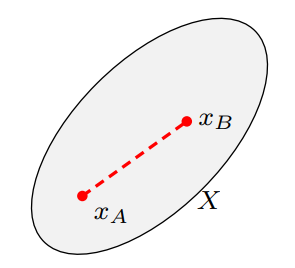
\includegraphics[width=0.4\linewidth]{cvxset}
    \caption{Convex set}
    \end{minipage}%
    \begin{minipage}{.5\textwidth}
        \centering
        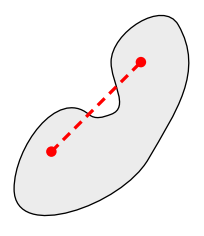
\includegraphics[width=0.4\linewidth]{ncvxset}
    \caption{Non convex set}
    \end{minipage}
\end{figure}

\subsubsection{Convex functions}
Let $X \subset \R^n$ be a convex set. A function $\ell:X\to\R$ is convex if for any two points $x_A$ and $x_B$ in $X$ and for all $\lambda\in[0,1]$, then 
\[
    \ell(\lambda x_A + (1-\lambda)x_B)\leq \lambda\ell(x_A)+ (1-\lambda)\ell(x_B)
\]
\begin{figure}[h]
    \centering
    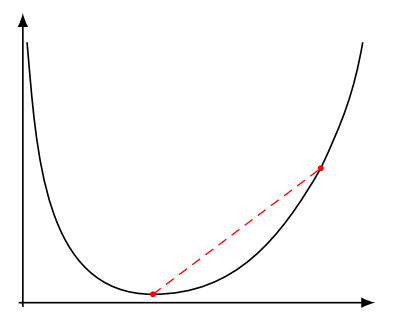
\includegraphics[width=0.35\textwidth]{cvxfcn}
    \caption{Convex function}
\end{figure}

A function $\ell$ is \emph{concave} if $-\ell$ is convex. A function $\ell$ is strictly convex if the inequality holds strictly for $x_A\neq x_B$ and $\lambda\in(0,1)$
\subsubsection{Inequality constraints and convex sets}
Let $g:\R^n\to\R^p$, we can define a set $X_{\text{ineq}}\subset \R^n$ as
\[
    X_{\text{ineq}} = \{x\in\R^n|g(x)\leq 0\}
\]
The set $X_{\text{ineq}}$ is convex iff $g$ is a quasi-convex function (e.g., monotone functions on the axis)
\subsubsection{Equality constraints and convex sets}
Let $h:\R^n\to\R^p$, we can define a set $X_{\text{eq}}\subset \R^n$ as
\[
    X_{\text{eq}} = \{x\in\R^n|h(x)= 0\}
\]
The set $X_{\text{eq}}$ is convex iff $h$ is an affine function. Convex sets identified through equality constraints are linear spaces (hyperplanes).



\subsection{Minimization of convex functions}
\subsubsection{Proposition}
Let $X\subset\R^n$ be a convex set and $\ell: X\to\R$ a convex function. Then a local minimum of $\ell$ is also a global minimum \\
Proof: not done in class but present in slides for funsies
\subsubsection{Necessary and sufficient condition of optimality (unconstrained)}
For the unconstrained minimization of a convex function it can be shown that the first order necessary condition of optimality is also sufficient (for a global minimum).
\subsubsection{Proposition}
Let $\ell:\R^n \to \R$ be a convex function. Then $x^*$ is a global minimum if and only if $\nabla\ell(x^*)=0$

Proof: not done in class but present in slides for funsies

\section{Quadratic programming (unconstrained)}
Let us consider a special class of optimization problems, namely quadratic optimization problems or quadratic programs: 
\[
    \min_{x\in\R^n}x^TQx+b^Tx
\]
with $Q=Q^T\in\R^{n\times n}$ and $b\in\R^n$


\subsubsection{optimality conditions}
First-order necessary condition for optimality: if $x^*$ is a minimum then 
\[
    \nabla \ell(x^*)=0 \implies 2Qx^*+b=0
\]
Second-order necessary condition for optimality: if $x^*$ is a minimum then 
\[
    \nabla^2\ell(x^*)\geq 0 \implies 2Q\geq0
\]
A necessary condition for the existence of minima for a quadratic program is that $Q\geq 0$. Thus, quadratic programs admitting at least a minimum are convex optimization problems.


\subsubsection{properties}
Since quadratic programs are convex programs ($Q\geq 0$ is necessary to have a local minimum), then the following holds: 
\begin{center}
     For a quadratic program necessary conditions of optimality are also sufficient and minima are global
\end{center}
If $Q>0$, then there exists a unique global minimum given by 
\[
    x^* = -\displaystyle\frac{1}{2}Q^{-1}b
\]


\section{Unconstrained Optimization Algorithms}
\subsection{Iterative descent methods}
We consider optimization algorithms relying on the iterative descent idea. We denote $x^k\in\R^n$ an estimate of a local minimum at iteration $k\in\N$. The algorithm starts at a given initial guess $x^0$ and iteratively generates vectors $x^1,x^2,\dots$ such that $\ell$ is decreased at each iteration, i.e. 
\[
    \ell(x^{k+1})<\ell(x^k) \qquad k = 1,2,\dots
\]
\subsubsection{two-step procedure}
We consider a general two-step procedure that reads as follows 
\[
    x^{k+1} = x^k+\gamma^k d^k, \qquad k=1,2,\dots
\]
in which 
\begin{enumerate}
    \item each $\gamma^k>0$ is a "step-size" 
    \item $d^k\in\R^n$ is a "direction"
\end{enumerate}
The goal is to 
\begin{enumerate}
    \item choose a direction $d^k$ along which the cost decreases for $\gamma^k$ sufficiently small;
    \item select a step-size $\gamma^k$ guaranteeing a sufficient decrease. 
\end{enumerate}
In other references these are called line-search methods.
\subsection{Gradient methods}
Let $x^k$ be such that $\nabla\ell(x^k)\neq 0$. We start by considering the update rule 
\[
    x^{k+1} = x^k-\gamma^k\nabla\ell(x^k)
\]
i.e., we choose $d^k = -\nabla\ell(x^k)$

From the first order Taylor expansion of $\ell$ at $x$ we have 
\begin{align*}
    \ell(x^{k+1}) & =  \ell(x^k)+\nabla\ell(x^k)^T(x^{k+1}-x^k)+o(\|x^{k+1}-x^k\|)\\
    & =  \ell(x^k)-\gamma^k\|\nabla\ell(x^k)\|^2+o(\gamma^k)
\end{align*}
Thus, for $\gamma^k>0$ sufficiently small it can be shown that $\ell(x^k+1)<\ell(x^k)$

The update rule 
\[
    x^{k+1}=x^k-\gamma^k\nabla\ell(x^k)
\]
can be generalized to so called \emph{gradient methods}
\[
    x^{k+1}=x^k+\gamma^kd^k
\]
with $d^k$ such that
\[
    \nabla\ell(x^k)^Td^k<0
\]
Also, $d^k$ must be gradient related, i.e. $d^k$ must not asymptotically become perpendicular to $\nabla\ell$
\subsubsection{selecting the descent direction}
Several gradient methods can be written as 
\[
    x^{k+1} = x^k-\gamma^kD^k\nabla\ell(x^k) \quad k=1,2,\dots
\]
where $D^k\in\R^{n\times n}$ is  a symmetric positive definite matrix. It can be immediately seen that 
\[
    -\nabla\ell(x^k)^TD^k\nabla\ell(x^k)<0
\]
i.e. $d^k = -D^k\nabla\ell(x^k)$ is a descent direction. The choice of $D^k$ must be made such that there exist $d_1,d_2$ positive real, such that $d_1 I \leq D^k \leq d_2 I$

Some choices for $D^k$:
\begin{itemize}
    \item Steepest descent $D^k=I_n$
    \item Newton's method $D^k = (\nabla^2\ell(x^k))^{-1}$\\
        It can be used when $\nabla^2\ell(x^k)>0$. It typically converges very fast asymptotically. For $\gamma^k = 1$ pure Newton's method
    \item Discretized Newton's method $D^k=(H(x^k))^{-1}$, where $H(x^k)$ is a positive definite symmetric approximation of $\nabla^2\ell(x^k)$ obtained by using finite difference approximations of the second derivatives 
    \item Some regularized version of the Hessian
\end{itemize}
\subsection{gradient method}
The update rule obtained for $D^k=I$ is called steepest descent. The name steepest descent is due to the following property: the normalized negative gradient direction 
\[
    d^k = -\displaystyle\frac{\nabla\ell(x^k)}{\|\nabla\ell(x^k)\|}
\]
minimizes the slope $\nabla \ell(x^k)^Td^k$ among all normalized directions, i.e. it gives the steepest descent.

\subsection{Newton's method for root finding}
Consider the nonlinear root finding problem 
\[
    r(x) = 0
\]
Idea: iteratively refine the solution such that the improved guess $x^{k+1}$ represents a root of the linear approximation of $r$ about the current tentative solution $x^k$. Consider the linear approximation of $r$ about $x^k$, we have 
\[
    r^k(x^k+\Delta x^k) = r(x^k)+\nabla r(x^k)^T\Delta x^k
\]
then, finding the zeros of the approximation, we have
\[
    \Delta x^k = -(\nabla r(x^k)^T)^{-1}r(x^k)
\]
Thus, the solution is improved as 
\[
    x^{k+1} = x^k-(\nabla r(x^k)^T)^{-1}r(x^k)
\]
\subsection{Newton's method for unconstrained optimization}
Consider the unconstrained optimization problem 
\[
    \min_{x\in\R^n} \ell(x)
\]
stationary points $\bar{x}$ satisfy the first order optimality condition 
\[
    \nabla \ell (\bar{x}) = 0
\]
We can look at it as a root finding problem, with $r(x)=\nabla\ell(x)$, and solve it via Newton's method. Therefore, we can compute $\Delta x^k$ as the solution of the linearization of $r(x)=\nabla\ell(x)$ at $x^k$, i.e. 
\[
    \nabla \ell(x^k) + \nabla^2\ell(x^k)\Delta x^k = 0
\]
and run the update 
\[
    x^{k+1} = x^k -(\nabla^2\ell(x^k))^{-1}\nabla\ell(x^k)
\]
We can introduce a variable step-size 
\[
    x^{k+1} = x^k-\gamma^k(\nabla^2\ell(x^k))^{-1}\nabla\ell(x^k)
\]
This is called generalized Newton's method
\subsubsection{Newton's method via Quadratic Optimization}
Observe that 
\[
    \nabla\ell(x^k) +\nabla^2\ell(x^k)\Delta x^k = 0
\]
is the first-order necessary and sufficient condition of optimality for the quadratic program 
\begin{equation}
    \label{qp}
    \Delta x^k = \argmin_{\Delta x}\nabla\ell(x^k)^T \Delta x+\displaystyle\frac{1}{2}\Delta x^T\nabla^2\ell(x^k)\Delta x
\end{equation}
Thus, the $k$-th iteration of Newton's method can be seen as 
\[
    x^{k+1} = x^k+\Delta x^k
\]
with $\Delta x^k$ solution of the quadratic problem \eqref{qp}. Generalized version: 
\[
    x^{k+1} = x^k + \gamma^k \Delta x^k
\]

\subsection{Gradient methods via quadratic optimization}
Similarly to Newton's method, a descent direction $\Delta x^k=D^k\nabla\ell(x^k)$ can be seen as the direction that minimizes at each iteration a different quadratic approximation of $\ell$ about $x^k$. In fact, consider the quadratic approximation $\ell^k(x)$ of $ \ell$ about $x^k$ given by 
\[
    \ell^k(x) = \ell(x^k)+\nabla\ell(x^k)^T(x-x^k)+\displaystyle\frac{1}{2}(x-x^k)^T(D^k)^{-1}(x-x^k)
\]
By setting the derivative to zero, we have 
\[
    \nabla\ell(x^k)+(D^k)^{-1}(x-x^k)=0
\]
we can calculate the minimum of $\ell^k(x)$ and set it as the next iterate $x^{k+1}$
\[
    \Delta x^k = -D^k\nabla\ell(x^k)
\]
\subsection{step-size selection rules}
\begin{itemize}
    \item Constant step-size: $\gamma^k=\gamma>0$
    \item Diminishing step-size: $\gamma^k\to 0$ as $k\to\infty$. It must hold that \[
            \displaystyle\sum_{k=0}^{\infty}\gamma^k = +\infty \quad \text{and} \quad \displaystyle\sum_{k=0}^{\infty}(\gamma^k)^2 < +\infty
        \]
        The above conditions avoid pathological choices of $\gamma^k$
    \item minimization rule
    \item Armijo rule
\end{itemize}

\subsection{Armijo rule}
Given the descent direction $d^k$ we can consider 
\[
    g^k(\gamma) = \ell(x^k+\gamma d^k), \quad g:\R\to\R
\]
% TODO insert image slide 30
The value of $g^k(\gamma)$ for $\gamma=0$ is $\ell(x^k)$. The minimization rule chooses as the value for $\gamma$ the value that minimizes $g^k(\gamma)$. The partial minimization rule would search for a minimum in a restricted set of values for $\gamma$. Let us differentiate $g$ wrt $\gamma$:
\begin{gather*}
    g'(\gamma)=\displaystyle\frac{d}{d\gamma}g(\gamma)=\displaystyle\frac{d}{d\gamma}\ell(x^k+\gamma d^k)\\
    g'(0) = \displaystyle\frac{d}{d\gamma}\at{\ell(x^k+\gamma d^k)}{\gamma=0} = \nabla \ell(x^k)^Td^k\\
\end{gather*}
We compute a linear approximation of $g(\gamma)$:
\begin{gather*}
    g(\gamma) = g(0) + g'(0)\gamma+o(\gamma)\\
    \ell(x^k+\gamma d^k) = \ell(x^k)+\gamma \nabla\ell(x^k)^Td^k + o(\gamma)
\end{gather*}
This is the tangent to the $g(\gamma)$ curve at $\gamma=0$. We also consider the line 
\[
    \ell(x^k)+c\gamma\nabla\ell(x^k)^Td^k
\]
which is a line with a slightly less negative slope given that $c\in(0,1)$.
The Armijo rule is applied as follows: 
\begin{enumerate}
    \item Set $\bar{\gamma}^0>0,\quad\beta\in(0,1),\quad c\in(0,1)$
    \item While $\ell(x^k+\bar{\gamma}^id^k)\geq \ell(x^k)+c\bar{\gamma}^i\nabla\ell(x^k)^Td^k$:
        \[
            \bar{\gamma}^{i+1}=\beta\bar{\gamma}^i
        \]
    \item Set $\gamma^k = \bar{\gamma}^i$
\end{enumerate}
Typical values are $\beta=0.7$ and $c=0.5$

\begin{figure}[h]
    \centering
    \begin{minipage}{.33\textwidth}
        \centering
        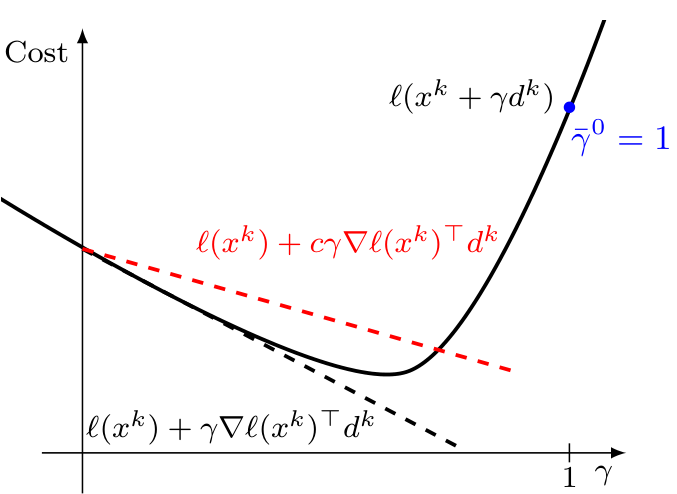
\includegraphics[width=0.9\linewidth]{armijo0}
    \end{minipage}%
    \begin{minipage}{.33\textwidth}
        \centering
        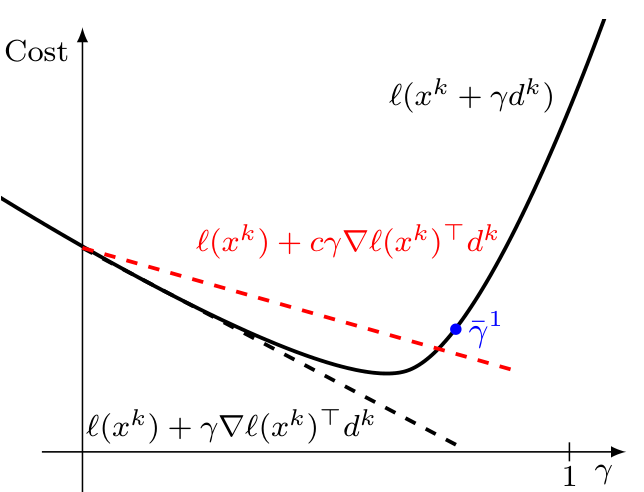
\includegraphics[width=0.9\linewidth]{armijo1}
    \end{minipage}%
    \begin{minipage}{.33\textwidth}
        \centering
        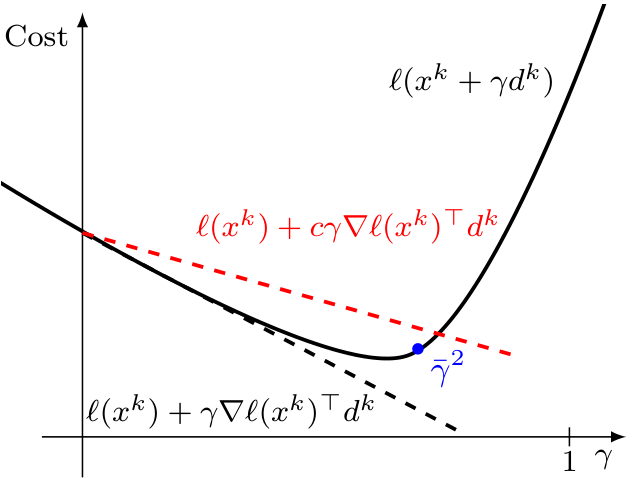
\includegraphics[width=0.9\linewidth]{armijo2}
    \end{minipage}%
\end{figure}

\subsubsection{Proposition: convergence with Armijo step-size}
Let $\{x^k\}$ be a sequence generated by a gradient method $x^{k+1}=x^k-\gamma^kD^k\nabla\ell(x^k)$ with $d_1I\leq D^k \leq d_2I, \quad d_1,d_2>0$. Assume that $\gamma^k$ is chosen by the Armijo rule and $\ell(x)\in \mathcal{C}^1$. Then, every limit point $\bar{x}$ of the sequence $\{x^k\}$ is a stationary point, i.e. $\nabla\ell(\bar{x})=0$
\begin{remark}
Recall that a vector $x\in\R^n$ is a limit point of a sequence $\{x^k\}$ in $\R^n$ if there exists a subsequence of $\{x^k\}$ that converges to $x$.
\end{remark}
\subsubsection{Convergence with constant or diminishing step-size}
Let $\{x^k\}$ be a sequence generated by a gradient method $x^{k+1}=x^k-\gamma^kD^k\nabla\ell(x^k)$ with $d_1I\leq D^k \leq d_2I, \quad d_1,d_2>0$. Assume that for some $L>0$ 
\[
    \|\nabla\ell(x)-\nabla\ell(y)\|\leq L\|x-y\|, \qquad \forall x,y\in\R^n
\]
i.e. The gradient is a Lipschitz continuous function.
Assume either
\begin{enumerate}
    \item $\gamma^k=\gamma>0$ sufficiently small, or 
    \item $\gamma^k\to 0$ and $\displaystyle\sum_{t=0}^{\infty}\gamma^k=\infty$
\end{enumerate}
Then, every limit point $\bar{x}$ of the sequence $\{x^k\}$ is a stationary point, i.e. $\nabla\ell(\bar{x})=0$

\subsubsection{Remarks on gradient methods}
\begin{itemize}
    \item The propositions do not guarantee that the sequence converges and not even existence of limit points. Then either $\ell(x^k)\to-\infty$ or $\ell(x^k)$ converges to a finite value and $\nabla\ell(x^k)\to 0$. In the second case, one can show that any subsequnce $\{x^{k_p}\}$ converges to some stationary point $\bar{x}$ satisfying $\nabla\ell(\bar{x})=0$
    \item Existence of minima can be guaranteed by excluding $\ell(x^k)\to-\infty$ via suitable assumptions. Assume, e.g., $\ell$ coercive (radially unboundend)
    \item For general (nonconvex) problems, assuming coercivity, only convergence (of subsequences) to stationary points can be proven.
    \item for convex programs, assuming coercivity, convergence to global minima is guaranteed since necessary conditions of optimality are also sufficient.
\end{itemize}

\section{Constrained optimization over convex sets}
Consider the optimization problem 
\[
    \min_{x\in X}\ell(x)
\]
where $X \subset \R^n$ is nonempty, convex, and closed, and $\ell$ is continuously differentiable on $X$. 
\subsubsection{Optimality conditions}
If a point $x^* \in X$ is a local minimum of $\ell(x)$ over $X$, then 
\[
    \nabla\ell(x^*)^T(\bar{x}-x^*)\geq 0 \qquad \forall\bar{x}\in X
\]
\subsubsection{Projection over a convex set}
Given a point $x\in\R^n$ and a closed convex set $X$, it can be shown that 
\[
    P_X(x) := \argmin_{z\in X}\|z-x\|^2
\]
exists and is unique. The point $P_X(x)$ is called the projection of $x$ on $X$.
\subsection{Projected gradient method}
Gradient methods can be generalized to optimization over convex sets 
\[
    x^{k+1}=P_X(x^k-\gamma^k\nabla\ell(x^k))
\]
The algorithm is based on the idea of generating at each $t$ feasible points (i.e. belonging to $X$) that give a descent in the cost. The analysis follows similar arguments to the one of unconstrained gradient methods.

\subsection{Feasible direction method}
Find $\tilde{x}\in\R^n$ such that 
\[
    \tilde{x} = \argmin_{x\in X} \ell(x^k)+\nabla\ell(x^k)^T(x-x^k)+\displaystyle\frac{1}{2}(x-x^k)^T(x-x^k)
\]
Update the solution 
\[
    x^{k+1}=x^k+\gamma^k(\tilde{x}-x^k)
\]
where $(\tilde{x}-x^k)$ is a feasible direction as it is contained in the set by construction. For $\gamma^k$ sufficiently small, $x^{k+1}\in X$

\subsubsection{Barrier function strategy for inequality constraints}
Consider the inequality constrained optimization problem 
\begin{align*}
    &\min_{x\in\R^d}\ell(x)\\
    \text{subj. to } &g_j(x)\leq 0 \quad j\in \{1,\dots,r\}
\end{align*}  
inequality constraints can be relaxed and embedded in the cost function by means of a barrier function $-\varepsilon \log(x)$. The resulting unconstraind problem reads as 
\[
    \min_{x\in\R^d} \ell(x) + \varepsilon \displaystyle\sum_{j=1}^{r}-\log(-g_j(x))
\]
Implementation: every few iterations shrink the barrier parameters $\varepsilon$

Methods such as this go by the name of \emph{interior point methods}

\section{Constrained optimization: optimality conditions}

\begin{align*}
    \min_{x\in X}\  &\ell(x)\\
    \text{subj. to } & g_j(x)\leq 0 \quad j\in\{1,\dots,r\}\\
    & h_i(x)=0 \quad i\in\{1,\dots,m\}
\end{align*}

\begin{definition}[Set of active inequality constraints]
    For a point $x$, the set of active inequality constraints at $x$ is $A(x) = \{j\in\{1,\dots,r\}|g_j(x)=0\}$
\end{definition}
\begin{definition}[Regular point]
    A point $x$ is regular if the vectors $\nabla h_i(x), i\in \{1,\dots,m\}$ and $\nabla g_j(x), j\in A(x)$, are linearly independent
\end{definition}
\subsubsection{Lagrangian function}
In order to state the first-order necessary conditions of optimality for (equality and inequality) constrained problems it is useful to introduce the Lagrangian function 
\[
    \mathcal{L}(x,\mu,\lambda)=\ell(x)+\displaystyle\sum_{j=1}^{r}\mu_ig_j(x) + \displaystyle\sum_{i=1}^{m}\lambda_i h_i(x)
\]
\begin{theorem}[Karush-Kuhn-Tucker necessary conditions]
    Let $x^*$ be a regular local minimum of 
    \begin{align*}
        \min_{x\in\R^d}\  &\ell(x) \\
        \text{subj. to }\  & g_j(x)\leq 0 \quad j\in\{1,\dots,r\}\\
        & h_i(x)=0 \quad i\in\{1,\dots,m\}
    \end{align*}
    where $\ell,g_j$ and $h_i$ are $\mathcal{C}^1$. \\
    Then $\exists!$  $\mu_j^*$ and $\lambda_i^*$, called \emph{Lagrange multipliers}, s.t.
    \[
        \begin{array}{ r c l}
            \nabla_1\mathcal{L}(x^*,\mu^*,\lambda^*) & = & 0 \\             \mu_j^* & \geq & 0 \\
            \mu^*_jg_j(x^*) & = & 0 \qquad j\in \{1,\dots,r\} 
        \end{array}
    \]
    Moreover, if $\ell, g_j$ and $h_i$ are $\mathcal{C}^2$ it holds
    \[
        y^T\nabla_{11}^2\mathcal{L}(x^*,\mu^*,\lambda^*)y \geq 0
    \]
    for all $y\in\R^n$ such that
    \[
    \nabla h_i(x)^Ty = 0, \quad i\in\{1,\dots,m\}, \qquad \nabla g_j(x)^Ty = 0, \quad j\in A(x) \quad \text{(i.e. } j\in\{1,\dots,r\} \text{ s.t. } g_j(x)=0\}
\]
\end{theorem}
\begin{remark}
    The condition $\mu^*g_j^*(x^*)=0,j\in\{1,\dots,r\}$, is called \emph{complementary slackness}
\end{remark}
\begin{notation}
    Points satisfying the KKT necessary conditions of optimality are referred to as \emph{KKT points}. They are the counterpart of stationary points in constrained optimization.
\end{notation}
\begin{notation}
    $\nabla_1$ denotes the gradient wrt the first variable of the function
\end{notation}
\begin{notation}
    $\nabla_{11}$ denotes the hessian of a function wrt the first variable
\end{notation}


\subsection{Quadratic programming (constrained)}
Let us consider quadratic optimization problems with linear equality constraints 
\begin{align*}
    \min_{x\in\R^n}\ & x^TQx+q^Tx \\
    \text{subj. to }\ & Ax=b
\end{align*}
with $Q=Q^T\in\R^{n\times n}, q\in\R^n, a\in\R^{m\times n}$ and $b\in\R^m$.
The Lagrangian function is:
\[
    \mathcal{L}(x,\lambda) = x^TQx + q^Tx +\displaystyle\sum_{i=1}^{m}\lambda_i(A_ix+b_i) =  x^TQx + q^Tx + \lambda^T(Ax-b)
\]
And the gradient computes as 
\[
    \nabla_1 \mathcal{L}(x^*,\lambda^*) = 2Qx^* + q + \displaystyle\sum_{i=1}^{m}\lambda_i^*A_i^T =  2Qx^* + q + A^T\lambda^*
\]
The equality constraints must also be enforced: 
\[
    Ax^*-b = 0
\]
We can note that 
\[
    \nabla_2\mathcal{L}(x^*,\lambda^*) = Ax-b
\]
Therefore, first order conditions of optimality may be written as 
\[
    \begin{bmatrix}
        \nabla_1\mathcal{L}(x^*,\lambda^*)\\ \nabla_2\mathcal{L}(x^*,\lambda^*)
    \end{bmatrix} = 0
\]
This is always the case when only equality constraints are present. Second order necessary conditions for optimality impose that, if $x^*$ is a minimum then 
\[
    y^T\nabla^2_{11}\mathcal{L}(x^*,\lambda^*)y = y^TQy \geq 0
\]
for all $y\in\R^n$ such that 
\[
    \nabla h_i(x)^T y = 0 \qquad i\in\{1,\dots,m\} \quad \implies \quad A^Ty = 0
\]
namely, for all $y\in\R^n$ in the null-space of $A^T$
\section{Constrained optimization: optimization algorithms}
\subsection{Newton's method for equality constrained problems}
KKT points can be found by solving a root finding problem in variables $x,\lambda$ wrt $r(x,\lambda)=\nabla \mathcal{L}(x,\lambda)$. Newton's method for this root finding problem reads as 
\[
    \begin{bmatrix}
        x^{k+1} \\ \lambda^{k+1}
        \end{bmatrix} = \begin{bmatrix}
        x^k \\ \lambda^k
        \end{bmatrix} + \begin{bmatrix}
        \Delta x^k \\ \Delta \lambda^k
    \end{bmatrix}
\]
with 
\[
    \begin{bmatrix}
        \Delta x^k \\ \Delta \lambda^k
    \end{bmatrix} = -(\nabla^2 \mathcal{L}(x^k,\lambda^k))^{-1}\nabla \mathcal{L}(x^k,\lambda^k)
\]
where 
\begin{gather*}
    \nabla^2\mathcal{L}(x^k,\lambda^k)= \begin{bmatrix}
        \nabla_{11} \mathcal{L}(x^*,\lambda^*) & \nabla_{12} \mathcal{L}(x^*,\lambda^*)\\
        \nabla_{21} \mathcal{L}(x^*,\lambda^*) & \nabla_{22} \mathcal{L}(x^*,\lambda^*)
        \end{bmatrix} = \begin{bmatrix}
        H^k & \nabla h(x^k) \\
        \nabla h(x^k)^T & 0
        \end{bmatrix} \\ \nabla \mathcal{L}(x^k,\lambda^k) = \begin{bmatrix}
        \nabla \ell(x^k)+\nabla h(x^k)\lambda^k \\ h(x^k)
    \end{bmatrix} \\
    H^k = \nabla_{11}^2 \mathcal{L}(x^k,\lambda^k) \qquad
    \nabla_{11}\mathcal{L}(x,\lambda) = \nabla^2 \ell(x) + \displaystyle\sum_{i=1}^{m}\lambda_i\nabla^2h_i(x)
\end{gather*}
We can write 
\[
    \nabla^2\mathcal{L}(x^k,\lambda^k)\begin{bmatrix}
        \Delta x^k \\ \Delta \lambda^k
    \end{bmatrix} = -\nabla \mathcal{L}(x^k,\lambda^k)
\]
namely 
\[
    \begin{bmatrix}
        H^k & \nabla h(x^k) \\
        \nabla h(x^k)^T & 0
        \end{bmatrix}  \begin{bmatrix}
        \Delta x^k \\ \Delta \lambda^k
        \end{bmatrix} = -\begin{bmatrix}
        \nabla \ell(x^k)+\nabla h(x^k)\lambda^k \\ h(x^k)
    \end{bmatrix}
\]
thus, $\Delta x^k, \Delta\lambda^k$ can be obtained as solution of a linear system of equations in the variables $\Delta x, \Delta\lambda$.
The linear system of equations can be rewritten as 
\begin{gather*}
    H^k\Delta x^k+\nabla h(x^k)\Delta \lambda^k = -\nabla\ell(x^k) - \nabla h(x^k)\lambda^k \\
    \nabla h(x^k)^T \Delta x^k = -h(x^k)
\end{gather*}
and equivalently as 
\begin{gather*}
    \nabla\ell(x^k) +H^k\Delta x^k+\nabla h(x^k)\Delta \lambda^{k+1} = 0 \\
    h(x^k)+\nabla h(x^k)^T\Delta x^k = 0
\end{gather*}
We can observe that the above equations are the necessary and sufficient optimality conditions for the Quadratic Program (QP)
\begin{align*}
    \min_{\Delta x}\  &\nabla\ell(x^k)^T\Delta x + \displaystyle\frac{1}{2}\Delta x^TH^k\Delta x \\
    \text{subj. to }\  & h(x^k) + \nabla h(x^k)^T \Delta x = 0
\end{align*}
Therefore, in the Newton's update, we can obtain $(\Delta x^k, \lambda^{k+1})$ by solving this QP.

\subsection{Sequential Quadratic Programming (SQP)}
Start from a tentative solution $x^0$. For $k=0,1,\dots$ (up to convergence)
\begin{enumerate}
    \item Compute $\nabla\ell(x^k),H^k,\nabla h(x^k)$ 
    \item Obtain ($\Delta x^k, \Delta \lambda^k_{QP}$) from 
        \begin{align}\label{sqp}
                \Delta x^k = \argmin_{\Delta x}\  & \nabla \ell(x^k)^T\Delta x +\displaystyle\frac{1}{2}\Delta x^TH^k \Delta x \\
                \text{subj. to }\  & h(x^k) + \nabla h(x^k)^T \Delta x = 0
        \end{align}
        with $\Delta\lambda^k_{QP}$ the Lagrange multiplier associated to the optimal solution of \eqref{sqp}
    \item Choose $\gamma^k$ using Armijo's rule on \emph{merit function} $M_1(x^k+\gamma\Delta x^k)$
    \item Update 
        \begin{gather*}
            x^{k+1} = x^k+ \gamma^k\Delta x^k \\
            \lambda^{k+1} = \Delta \lambda^*_{QP}
        \end{gather*}
\end{enumerate}

\subsection{Barrier function strategy for inequality constraints}
Consider the inequality optimization problem 
\begin{align*}
    \min_{x\in\R^d} & \ell(x) \\
    \text{subj. to } & g_j(x) \leq 0 \qquad j\in\{1,\dots,r\}\\
    & h(x) = 0
\end{align*}
Inequality constraints can be embedded in the cost function by means of a \emph{barrier function} $-\varepsilon \log(x)$. The resulting unconstrained problem reads as 
\begin{gather*}
    \min_{x\in\R^d}\ell(x) + \varepsilon\displaystyle\sum_{j=1}^{r}-\log(-g_j(x)) \\
    h(x) = 0
\end{gather*}
Implementation: every few iterations shrink the barrier parameters $\varepsilon$



\chapter{Optimality conditions for optimal control}
\section{boh}
\subsection{Dynamics as equality constraints}
We consider nonlinear, discrete-time systems described by 
\begin{equation} \label{system2}
    x_{t+1} = f_t(x_t,u_t) \qquad t\in\N_0
\end{equation}
Let us rewrite the nonlinear dynamics of a dt system as an implicit equality constraint $h:\R^{nT}\times \R^{mT}\to\R^{nT}$ 
\[
    h\traj:=\begin{bmatrix}
        f_0(x_0,u_0)-x_1 \\ \vdots \\ f_{T-1}(x_{T-1},u_{T-1})-x_T
    \end{bmatrix}
\]
so that a curve $\traj$ is a trajectory of the system if it satisfies the (possibly nonlinear) equality constraint 
\[
    h\traj = 0
\]
\subsection{system trajectories and trajectory manifold}
We can now define the trajectory manifold $\mathcal{T}\subset \R^{nT}\times \R^{mT}$ of \eqref{system2}
\begin{align*}
    \mathcal{T} := &\left\{\left(\mathbf(x),\mathbf(u)\right)\in\R^{nT}\times\R^{mT}|h\left(\mathbf(x),\mathbf(u)\right)=0\right\}\\=&\left\{\left(\mathbf(x),\mathbf(u)\right)\in\R^{nT}\times\R^{mT}|x_{t+1}=f_t\left(x_t,u_t\right),t=0,\dots,T-1\right\}
\end{align*}
Let $\traj\in\mathcal{T}$ be a trajectory of the system, i.e. a point on the trajectory manifold $\mathcal{T}$. The tangent space to $\mathcal{T}$ at a given trajectory (point) $\traj$, denoted as $T_{(\bar{\mathbf{x}},\bar{\mathbf{u}})}\mathcal{T}$, is the set of trajectories satisfying the linearization of $x_{t+1} = f_t(x_t,u_t)$ about the trajectory $(\bar{\mathbf{x}},\bar{\mathbf{u}})$.
That is, $T_{(\bar{\mathbf{x}},\bar{\mathbf{u}})}\mathcal{T}=\{(\mathbf{\Delta x, \Delta u})\in\R^{nT}\times\R^{mT}|\nabla_1h(\mathbf{x},\mathbf{u})^T\mathbf{\Delta x} + \nabla_2h(\mathbf{x},\mathbf{u})^T\mathbf{\Delta u} = 0\}$ is the set of trajectories $(\mathbf{\Delta x, \Delta u})$ of
\[
    \Delta x_{t+1} = A_t\Delta x_t + B_t \Delta u_t
\]
with 
\begin{gather*}
    A_t = \nabla_1f_t(\bar{x}_t,\bar{u}_t)^T\\
    B_t = \nabla_2f_t(\bar{x}_t,\bar{u}_t)^T
\end{gather*}


\section{Unconstrained optimal control problem (d-t)}
We look for a solution of the discrete-time optimal control problemm 
\begin{align*}
        \min_{\mathbf{x}\in\R^n,\mathbf{u}\in\R^m} & \displaystyle\sum_{t=0}^{T-1}\ell_t(x_t,u_t)+\ell_T(x_T)\\
        \text{subj. to } & x_{t+1} = f_t(x_t,u_t), \quad t\in\{0,\dots,T-1\} 
\end{align*}
with given initial condition $x_0 = x_{\text{init}}\in \R^n$. 

From now on, we will assume that functions $\ell_t(\cdot,\cdot),\ell_T(\cdot),f_t(\cdot,\cdot)$ are twice continuosly differentiable, i.e. they are class $\mathcal{C}^2$
Consider the discrete-time system \eqref{system2}. We can introduce the compact notation 
\[
    \mathbf{x} := \begin{bmatrix}
        x_1 \\ \vdots \\ x_T
    \end{bmatrix} \qquad \mathbf{u} := \begin{bmatrix}
        u_0 \\ \vdots \\ u_{T-1}
    \end{bmatrix}
\]
which allows us to write the cost function compactly as 
\[
    \ell({\mathbf{x},\mathbf{u}}) := \sum_{t=0}^{T-1}\ell_t(x_t,u_t)+\ell_T(x_T)
\]
and the equality constraint represented by the dynamics 
\[
    h(\mathbf{x},\mathbf{u}) := \begin{bmatrix}
        f_0(x_0,u_0)-x_1 \\ \vdots \\ f_{T-1}(x_{T-1}u_{T-1})-x_T
    \end{bmatrix}
\]
In light of this compact notation, we can rewrite the optimal control law problem as 
\begin{align*}
    \min_{\mathbf{x}\in\R^{nT},\mathbf{u}\in\R^{mT}} &\ell(\mathbf{x},\mathbf{u})\\
    \text{subj. to } & h(\mathbf{x},\mathbf{u})=0
\end{align*}
where $\ell:\R^{nT}\times\R^{mT}\to\R$ and $h:\R^{nT}\times\R^{mT}\to\R^{nT}$. This is a constrained nonlinear optimization problem with decision variable $(\mathbf{x},\mathbf{u})$

\section{KKT conditions for unconstrained optimal control}
the Lagrangian function has the form 
\begin{align*}
    \mathcal{L}(\mathbf{x,u,\lambda}) &= \ell(\mathbf{x,u})+\boldsymbol{\lambda}^Th(\mathbf{x,u}) \\
    &= \displaystyle\sum_{t=0}^{T-1}\ell_t(x_t,u_t)+\ell_T(x_T) + \displaystyle\sum_{t=0}^{T-1}\lambda^T_{t+1}(f_t(x_t,u_t)-x_{t+1}) \\
    &= \displaystyle\sum_{t=0}^{T-1}\left(\ell_t(x_t,u_t)+\lambda^T_{t+1}(f_t(x_t,u_t)-x_{t+1})\right)+\ell_T(x_T) \\
    &=\displaystyle\sum_{t=0}^{T}\mathcal{L}_t(x_t,u_t,\boldsymbol{\lambda})
\end{align*}
where $\boldsymbol{\lambda}\in\R^{nT}$ and 
\begin{align*}
    \mathcal{L}_0(x_0,u_0,\boldsymbol{\lambda}) &= \ell_0(x_0,u_0)+\lambda_1^T f_0(x_0,u_0)\\
    \mathcal{L}_t(x_t,u_t,\boldsymbol{\lambda}) &= \ell_t(x_t,u_t)+\lambda_1^T f_t(x_t,u_t)-\lambda_tx_t\\
    \mathcal{L}_T(x_T,\boldsymbol{\lambda}) &= \ell_T(x_T) - \lambda_T^Tx_T
\end{align*}
Let $(\mathbf{x}^*,\mathbf{u}^*)$ be a regular point for the dynamics constraints and an optimal (state-input) trajectory. Then there exists $\boldsymbol{\lambda}^*$ such that $\nabla \mathcal{L}(\mathbf{x}^*,\mathbf{u}^*,\boldsymbol{\lambda}^*)=0$ 

Let us explicitly write condition $\nabla_{(1,2)} \mathcal{L}(\mathbf{x}^*,\mathbf{u}^*,\boldsymbol{\lambda}^*) = 0 $ 
\[
    \nabla_{(1,2)} \mathcal{L}(\mathbf{x}^*,\mathbf{u}^*,\boldsymbol{\lambda}^*) = \begin{bmatrix}
        \nabla_1\mathcal{L}(\mathbf{x}^*,\mathbf{u}^*,\boldsymbol{\lambda}^*)\\
        \nabla_2\mathcal{L}(\mathbf{x}^*,\mathbf{u}^*,\boldsymbol{\lambda}^*)
    \end{bmatrix} = 0
\]
Let us note that 
\[
    \nabla_1\mathcal{L}(\mathbf{x}^*,\mathbf{u}^*,\boldsymbol{\lambda}^*) = \at{\begin{bmatrix}
            \displaystyle\frac{\partial \mathcal{L}(\mathbf{x},\mathbf{u},\boldsymbol{\lambda})}{\partial (x_1)_1}\\
            \vdots \\
            \displaystyle\frac{\partial \mathcal{L}(\mathbf{x},\mathbf{u},\boldsymbol{\lambda})}{\partial (x_1)_n}\\
            \vdots \\
            \displaystyle\frac{\partial \mathcal{L}(\mathbf{x},\mathbf{u},\boldsymbol{\lambda})}{\partial (x_T)_1}\\
            \vdots \\
            \displaystyle\frac{\partial \mathcal{L}(\mathbf{x},\mathbf{u},\boldsymbol{\lambda})}{\partial (x_T)_n}
    \end{bmatrix}}{\mathbf{x}=\mathbf{x}^*}
\]
Since $\mathcal{L}(\mathbf{x},\mathbf{u},\boldsymbol{\lambda})= \displaystyle\sum_{t=0}^{T}\mathcal{L}(x_t,u_t,\boldsymbol{\lambda})$, we can exploit this sparsity and write 
\begin{align*}
    \nabla_2\mathcal{L}_0(x_0,u_0,\boldsymbol{\lambda}) = 0 \qquad & \nabla_2\ell_0(x_0,u_0)\nabla_2f_0(x_0,u_0)\lambda_0\\
    \begin{bmatrix}
        \nabla_1\mathcal{L}_t(x_t,u_t,\boldsymbol{\lambda})\\
        \nabla_2\mathcal{L}_t(x_t,u_t,\boldsymbol{\lambda})
    \end{bmatrix} = 0 \qquad &  
    \begin{bmatrix}
        \nabla_1\ell_t(x_t,u_t) + \nabla_1f_t(x_t,u_t)\lambda_{t+1}-\lambda_t \\
        \nabla_2\ell_t(x_t,u_t) + \nabla_2f_t(x_t,u_t)\lambda_{t+1}
    \end{bmatrix} = 0 \quad t=1,\dots,T-1 \\
    \nabla_1\mathcal{L}_t(x_t,\boldsymbol{\lambda}) = 0\qquad & \nabla\ell_T(x_T)-\lambda_T = 0
\end{align*}
Let us introduce some notation: 
\begin{gather*} 
    \nabla_1\ell_t(x_t^*,u_t^*) = a_t\in \R^n\\
    \nabla_1f_t(x_t^*,u_t^*) = A_t^T\\
    \nabla_2\ell_t(x_t^*,u_t^*) = b_t\in \R^n\\
    \nabla_2f_t(x_t^*,u_t^*) = B_t^T
\end{gather*}
So we can rewrite the KKT conditions for unconstrained optimal control as:
\begin{flalign*}
    &\lambda_t^* = A_t^T\lambda_{t+1}^* + a_t \qquad t= T-1,\dots,1\\
    &\lambda_T^* = \nabla\ell(x_T^*)\\
    &B_t^T\lambda_{t+1}^* + b_t = 0 \qquad t=0,\dots,T-1 
\end{flalign*}

\subsection{Indirect methods for optimal control}
Based on solving the optimality conditions: 
\begin{itemize} % TODO look in recording
    \item Guess some $u_t^0,\quad t= 0,\dots,T-1 \quad k=0$ 
    \item run "forward" 
        \[
            x_{t+1}^0 = f_t(x_t^0,u_t^0) \quad x_0
        \]
    \item run "backward"
        \[
            a
        \]
    \item given $\lambda_t^0 \quad t=1,\dots,T$ solve:
        \[
            \nabla_2\ell(x_t^0,u_t) + \nabla_2f(x_t^0,u_t)\lambda_{t+1}^0 = 0 \quad t=0,\dots,T-1
        \]
        to get $u_{t}^1 \quad t=0,\dots,T-1$
\end{itemize}


\section{KKT conditions for constrained optimal control}
We look for a solution of the discrete-time optimal control problem
\begin{align*}
        \min_{x_0\in\R^n,\mathbf{x}\in\R^{nT},\mathbf{U}\in\R^{mT}} & \displaystyle\sum_{t=0}^{T-1}\ell_t(x_t,u_t)+\ell_T(x_T) \\
        \text{subj. to } & x_{t+1} = f_t(x_t,u_t), \quad t=0,\dots,T-1\\
                        & r(x_0,x_T) = 0 \\
                        & g_t(x_t,u_t)\leq 0 ,\quad t=0,\dots,T-1
\end{align*}
where 
\begin{itemize}
    \item $\ell_t:\R^n\times\R^m\to\R$ is the stage cost,
    \item $\ell_T:\R^n\to\R$ is the terminal cost,
    \item $r: \R^n\times\R^n\to\R^{p_0}$ identifies a \emph{boundary constraint} on initial and final states,
    \item $g_t:\R^n\times\R^m\to\R^p$ for each $t$ identifies \emph{point-wise constraints} on state and input at some time $t$
\end{itemize}
The Lagrangian function has the form 
\begin{align*}
    \mathcal{L}(\mathbf{x},\mathbf{u},\boldsymbol{\lambda},\mathbf{\mu}) =& \ell(\mathbf{x},\mathbf{u})+\boldsymbol{\lambda}_d^T h(\mathbf{x},\mathbf{u})+ \lambda_b^T r(x_0,x_T) + \mathbf{\mu}^Tg(\mathbf{x},\mathbf{u}) \\ 
    =&\displaystyle\sum_{t=0}^{T-1}\ell_t(x_t,u_t)+\ell_T(x_T) + \displaystyle\sum_{t=0}^{T-1}\lambda_{d,t+1}(f_t(x_t,u_t)-x_{t+1})+\lambda_b^Tr(x_0,x_T) + \displaystyle\sum_{t=0}^{T-1}\mu_t^Tg_t(x_t,u_t)\\
    =&\displaystyle\sum_{t=0}^{T}\mathcal{L}_t(x_t,u_t,\boldsymbol{\lambda},\mathbf{\mu})
\end{align*}
where
\begin{align*}
    \mathcal{L}_0(x_0,u_0,\boldsymbol{\lambda},\boldsymbol{\mu}) &= \ell_0(x_0,u_0)+\lambda_{d,1}^T f_0(x_0,u_0) + \lambda_{b,0}r_0(x_0)\\
    \mathcal{L}_t(x_t,u_t,\boldsymbol{\lambda}) &= \ell_t(x_t,u_t)+\lambda_1^T f_t(x_t,u_t)-\lambda_tx_t+\mu_t^Tg_t(x_t,u_t)\\
    \mathcal{L}_T(x_T,\boldsymbol{\lambda}) &= \ell_T(x_T) - \lambda_T^Tx_T + \lambda_{b,T}^Tr_T(x_T)
\end{align*}
and we assumed $r(x_0,x_T)=\col(r_0(x_0),r_T(x_T))$ and $\lambda_b = \col(\lambda_{b,0},\lambda_{b,T})$.

Let $(\mathbf{x}^*,\mathbf{u}^*)$ be a regular point for the dynamics constraints and an optimal (state-input) trajectory. Then there exists $\boldsymbol{\lambda}^*$ such that $\nabla \mathcal{L}(\mathbf{x}^*,\mathbf{u}^*,\boldsymbol{\lambda}^*)=0$ 

Let us explicitly write condition $\nabla_{(1,2)} \mathcal{L}(\mathbf{x}^*,\mathbf{u}^*,\boldsymbol{\lambda}^*,\boldsymbol{\mu}^*) = 0 $ 
\[
    \nabla_{(1,2)} \mathcal{L}(\mathbf{x}^*,\mathbf{u}^*,\boldsymbol{\lambda}^*,\boldsymbol{\mu}^*) = \begin{bmatrix}
        \nabla_1\mathcal{L}(\mathbf{x}^*,\mathbf{u}^*,\boldsymbol{\lambda}^*,\boldsymbol{\mu}^*)\\
        \nabla_2\mathcal{L}(\mathbf{x}^*,\mathbf{u}^*,\boldsymbol{\lambda}^*,\boldsymbol{\mu}^*)
    \end{bmatrix} = 0
\]
Since $\mathcal{L}(\mathbf{x},\mathbf{u},\boldsymbol{\lambda}^*,\boldsymbol{\mu}^*)= \displaystyle\sum_{t=0}^{T}\mathcal{L}(x_t,u_t,\boldsymbol{\lambda})$, we can exploit this sparsity and write 
\begin{align*}
    \begin{bmatrix}
        \nabla_1\mathcal{L}_0(x_0,u_0,\boldsymbol{\lambda},\boldsymbol{\mu}) \\
        \nabla_2\mathcal{L}_0(x_0,u_0,\boldsymbol{\lambda},\boldsymbol{\mu}) 
    \end{bmatrix} = 0 \qquad &
    \begin{bmatrix}
        \nabla_1\ell(x_0,u_0)\nabla_1f_0(x_0,u_0)\lambda_1+\nabla r_0(x_0)\lambda_{b,0}+\nabla_1g_t(x_0,\mu_0)\\
        \nabla_2\ell_0(x_0,u_0)\nabla_2f_0(x_0,u_0)\lambda_1 + \nabla_2g_t(x_0,u_0)\mu_0\\
    \end{bmatrix} = 0\\
    \begin{bmatrix}
        \nabla_1\mathcal{L}_t(x_t,u_t,\boldsymbol{\lambda})\\
        \nabla_2\mathcal{L}_t(x_t,u_t,\boldsymbol{\lambda})
    \end{bmatrix} = 0 \qquad &  
    \begin{bmatrix}
        \nabla_1\ell_t(x_t,u_t) + \nabla_1f_t(x_t,u_t)\lambda_{t+1}-\lambda_t + \nabla_1g_t(x_t,u_t)\mu_t\\
        \nabla_2\ell_t(x_t,u_t) + \nabla_2f_t(x_t,u_t)\lambda_{t+1} + \nabla_2g_t(x_t,u_t)\mu_t
    \end{bmatrix} = 0 \quad t=1,\dots,T-1 \\
    \nabla_1\mathcal{L}_t(x_t,\boldsymbol{\lambda}) = 0\qquad & \nabla\ell_T(x_T)-\lambda_T + \nabla r_T(x_T)\lambda_{b,T} = 0
\end{align*}
for $(x_t,u_t,\lambda_t,\mu_t) = (x_t^*,u_t^*,\lambda_t^*,\mu_t^*)$

















\chapter{Linear Quadratic (LQ) optimal control}

Consider a linear quadratic optimal control problem as: 
\[
    \begin{array}{r l}
        \min_{\substack{x_1,\dots,x_T \\ u_0,\dots,u_{T-1}}} & \displaystyle\sum_{t=0}^{T-1}\displaystyle\frac{1}{2}[x_t^TQ_tx_t+u_t^TR_tu_t] + \displaystyle\frac{1}{2}x_T^TQ_Tx_T\\
        \text{subj. to} & x_{t+1} = A_tx_t + B_tu_t \quad t=0,\dots,T-1\\
                        &x_0 = x_{\text{init}}
    \end{array}
\]
We assume $Q_t=Q_t^T\geq 0,\ $ for $ t=0,\dots,T-1$, $Q_T = Q_T^T \geq 0$, and $R_t=R_t^T > 0 \ $ for $t=0,\dots,T-1$

\section{First order optimality condition}
\begin{gather*}
    \nabla_1f_t(x_t,u_t) = A_t^T\\
    \nabla_1\ell(x_t,u_t) = \nabla_1(\displaystyle\frac{1}{2}x_t^TQ_tx_t+\displaystyle\frac{1}{2}u_t^TR_tu_t)=Q_tx_t\\
    \nabla_2f_t(x_t,u_t) = B_t^T\\
    \nabla_2\ell_t(x_t,u_t) = R_tu_t\\
\end{gather*}
therefore 
\begin{gather*}
    \lambda_t^* = A_t^T\lambda_{t+1}^* + Q_tx_t^* \quad t= T_1,\dots,0\\
    \lambda_T^* = Q_Tx_T^* \\
    B_t^T\lambda_{t+1}^* + R_tu_t^* = 0 \quad t=0,\dots,T-1
\end{gather*}
\begin{remark}
second order optimality conditions 
\[
    y^T\nabla^2_{(1,2)(1,2)}\mathcal{L}(\mathbf{x}^*,\mathbf{u}^*,\boldsymbol{\lambda}^*,)y \geq 0
\]
For vectors $y$ satisfying the "linear approximation of the constraint". The hessian turns out as 
\[
    \begin{bmatrix}
        Q_1 & & &  0\\
            & \ddots & & & \\ 
        0 & & & Q_n
    \end{bmatrix}
\]
\end{remark}
Because $R_t>0$ it is invertible, we can write 
\[
    u_t^* = -R_t^{-1}B_t^T\lambda_{t+1}^*
\]
Introducing a matrix $P_t=P_t^T \geq 0$, it can be proven that 
\[
    \lambda_t^* = P_tx_t^*
\]
Assuming that it holds for some $t\leq T-1$, then we have 
\[
    u_t^* = -R_t^{-1}B_t^TP_{t+1}x_{t+1}^*
\]
Now, considering the constraint represented by the dynamics 
\[
    u_t^* = -R_t^{-1}B_t^TP_{t+1}(A_tx_t^*+B_tu_t^*)
\]
Solving by $u^*_t$ yields 
\[
    u_t^* = -(R_t+B_t^Tp_{t+1}B_t)^{-1}B_t^TP_{t+1}A_tx^*_t \quad t=0,\dots,T-1
\]
we get 
\begin{gather*}
    u_t^* = -R_t^{-1}B_t^Tp_{t+1}x_{t+1}^* \\
    = -R_t^{-1}B_t^TP_{t+1}(A_tx_t^*+B_tu_t^*)
\end{gather*}
we multiply both sides by $R_t$: 
\begin{gather*}
    R_tu_t^* = -B_t^TP_{t+1}(A_tx_t^*+B_tu_t^*)\\
    R_tu_t^* = -B_t^TP_{t+1}A_tx_t^*-B_t^TP_{t+1}B_tu_t^*\\
    (R_t+B_t^TP_{t+1}B_t)u_t^* = -B_t^TP_{t+1}A_tx_t^*
\end{gather*}
The matrix on the left is clearly positive definite, therefore: 
\[
    u_t^* = -(R_t+B_t^TP_{t+1}B_t)^{-1}B_t^TP_{t+1}A_tx_t^*
\]
which we can write as 
\[
    u_t^* = K_t^*x_t^*
\]
that is, the optimal control is a state feedback with gain $-(R_t+B_t^TP_{t+1}B_t)^{-1}B_t^TP_{t+1}$
\[
    x_{t+1}^* = A_tx_t^*-B_t(R_t+B_t^TP_{t+1}B_t)^{-1}B_t^TP_{t+1}A_tx_t^*
\]
which we can rewrite as 
\[
    x_{t+1}^* = (A_t-B_t(R_t+B_t^TP_{t+1}B_t)^{-1}B_t^TP_{t+1}A_t)x_t^*
\]
which is a closed loop system. We multiply both sides by $P_{t+1}$ and obtain 
\[
    P_{t+1}x_{t+1}^* = P_{t+1}(A_t-B_t(R_t+B_t^TP_{t+1}B_t)^{-1}B_t^TP_{t+1}A_t)x_t^*
\]
On the left side of the equation we have obtained $\lambda_{t+1}^*$
\[
    \lambda_{t+1}^* =P_{t+1}(A_t-B_t(R_t+B_t^TP_{t+1}B_t)^{-1}B_t^TP_{t+1}A_t)x_t^*
\]
Remembering that $\lambda_t^* = A_t^T\lambda_{t+1}^*+Q_tx_t^*$ we multiply both sides by $A_t^T$ and then add $Q_tx^*_t$ and obtain 
\[
    A_t^T\lambda_{t+1}^*+Q_tx_t^*=A_t^TP_{t+1}(A_t-B_t(R_t+B_t^TP_{t+1}B_t)^{-1}B_t^TP_{t+1}A_t)x_t^* + Q_tx_t^*
\]
and because 
\[
    \lambda_t^* = P_tx_t^*
\]
then 
\[
    P_tx_t^* = [A_t^TP_{t+1}(A_t-B_t(R_t+B_t^TP_{t+1}B_t)^{-1}B_t^TP_{t+1}A_t)+Q_t]x_t^*
\]
so 
\[
    P_tx_t^* = \left[A_t^TP_{t+1}A_t-A_t^TP_{t+1}B_t(R_t+B_t^TP_{t+1}B_t)^{-1}B_t^TP_{t+1}A_t+Q_t\right]x_t^*
\]
from which 
\begin{equation}\label{Riccati}
    P_t = A_t^TP_{t+1}A_t-A_t^TP_{t+1}B_t(R_t+B_t^TP_{t+1}B_t)^{-1}B_t^TP_{t+1}A_t+Q_t
\end{equation}
because $\lambda_T^*=Q_Tx_T^*$ we have that 
\[
    P_T = Q_T
\]
Therefore, by propagating equation \eqref{Riccati} back in time, $P_t$ can be calculated. Equation \eqref{Riccati} is called difference Riccati equation
\begin{itemize}
    \item gains $K_t^*$ can be precomputed offline and then used for different $x_0$ 
    \item It can be shown that if $T\to\infty$ the gains $K_t^*$ converge and asymptotically stabilize the system
\end{itemize}
\subsubsection{Other formulations of the Riccati equation}
The usual Riccati recursion reads:
\[
    P_t = Q_t + A_t^TP_{t+1}A_t - A_t^TP_{t+1}B_t(R_t+B_t^TP_{t+1}B_t)^{-1}B_t^TP_{t+1}A_t
\]
by exploiting the matrix inversion lemma\footnote{$(A+BC)^{-1} = A^{-1}-A^{-1}B(I+CA^{-1}B)^{-1}CA^{-1}$}, we can write: 
\begin{align*}
    P_t &= Q_t + A_t^TP_{t+1}A_t - A_t^TP_{t+1}B_t(R_t+B_t^TP_{t+1}B_t)^{-1}B_t^TP_{t+1}A_t\\
    P_t &= Q_t + A_t^TP_{t+1}(I-B_t(R_t+B_t^TP_{t+1}B_t)^{-1}B_t^TP_{t+1})A_t\\
    P_t &= Q_t + A_t^TP_{t+1}(I-B_t((I+B_t^TP_{t+1}B_tR_t^{-1})R_t)^{-1}B_t^TP_{t+1})A_t\\
    P_t &= Q_t + A_t^TP_{t+1}(I-B_tR_t^{-1}(I+B_t^TP_{t+1}B_tR_t^{-1})^{-1}B_t^TP_{t+1})A_t\\
    P_t &= Q_t + A_t^TP_{t+1}(I-B_tR_t^{-1}B_t^TP_{t+1})A_t\\
    P_t &= Q_t + A_t^T(I-B_tR_t^{-1}B_t^TP_{t+1})P_{t+1}A_t
\end{align*}
\section{Infinite horizion LQ optimal control}
Consider the infinite-horizon optimal control problem
\begin{align*}
        \min_{\substack{x_1,x_2,\dots \\ u_0,u_1,\dots}} & \displaystyle\sum_{t=0}^{\infty}\displaystyle\frac{1}{2}\left[x_t^TQx_t+u_t^TRu_t\right] \\
        \text{subj. to } & x_{t+1} = Ax_t + Bu_t \quad t=0,1,\dots\\
                        &x_0 = x_{\text{init}}
\end{align*}
where 
\begin{itemize}
    \item $x\in\R^n$ and $u\in\R^m$
    \item $A\in\R^{n\times n}$
    \item $B\in\R^{n\times m}$
    \item $Q\in\R^{n\times n}$ and $Q=Q^T\geq 0$
    \item $R\in\R^{m\times m}$ and $R=R^T> 0$
\end{itemize}
We assume the pair $(A,B)$ is controllable and the pair $(A,C)$ with $Q=C^TC$ is observable
Let us write 
\[
    y_t=Cx_t
\]
which leads to 
\[
    \displaystyle\frac{1}{2}x_t^TQx_t = \displaystyle\frac{1}{2}x_t^TC^TCx_t = \displaystyle\frac{1}{2}y_t^Ty_t
\]
The controllability assumption guardantees that an optimal controller exists: if $(A,B)$ controllable, then $\exists \bar{u}_0,\dots,\bar{u}_{T-1}$ for $T$ sufficiently large ($T=n$) such that $\forall x_0\in \R^n\implies x_T=0$. Consider the input
\[
    \bar{u}_0,\dots,\bar{u}_{T-1},0,\dots,0,\dots
\]
Let us compute the cost associated to this input 
\[
    \displaystyle\sum_{t=0}^{\infty}\displaystyle\frac{1}{2}[x_t^TQx_t+u_t^TRu_t] =\displaystyle\sum_{t=0}^{T-1}\displaystyle\frac{1}{2}\bar{x}_t^TQ\bar{x}_t + \displaystyle\frac{1}{2}\bar{u}_t^TR\bar{u}_t
\]
We can note that the cost is a finite quantity. Because the cost is finite, There must exist a solution which minimizes the cost.
\proposition

Let the pair $(A,B)$ be controllable and the pair $(A,C)$ with $Q=C^TC$ be observable. Then the following holds:
\begin{itemize}
    \item there exists a unique positive definite $P_\infty$ equilibrium solution of the Difference Riccati Equation. That is, $P_\infty$ is a solution of \[
            P_\infty = Q+A^TP_\infty A-A^TP\infty B(R+B^TP_\infty B)^{-1}B^TP_\infty A
        \]
        which is called \emph{Algebraic Riccati Equation }
        \item the optimal control is a feedback of the state given by:
            \begin{flalign*}
                & K^* = -(R+B^TP_\infty B)^{-1}(B^TP_\infty A)\\
                & u_t^* = K^*x^*_t\\
                & x_{t+1}^* = Ax_t^*+Bu_t^* \quad t=1,2,\dots \quad x_0^* = X_{\text{init}}
            \end{flalign*}
\end{itemize}
\remark The observability of $(A,C)$ guardantees that if the stage cost goes to zero, then the state trajectory goes to zero.







\chapter{Optimality Conditions for Unconstrained Optimal Control via Shooting}

Let us consider the system dynamics 
\[
    x_{t+1} = f_t(x_t,u_t) \quad t=0,\dots,T-1 \quad x_0 \text{ given}
\]
and let us suppose we have an input sequence $u_0,\dots,u_{T-1}$. We have: 
\begin{flalign*}
    & x_1 =f_0(x_0,u_0) = \tilde{\Phi}_1(\mathbf{u}) \\
    &  x_2 = f_1(x_1,u_1) = f_1(f_0(x_0,u_0),u_1) = \tilde{\Phi}_2(\mathbf{u}) \\
    & \vdots \\
    & x_t = \tilde{\Phi}_t(\mathbf{u}) \qquad t=0,\dots,T-1
    & \vdots \\
    & x_T = \tilde{\Phi}_{T}(\mathbf{u}) \qquad t=0,\dots,T-1
\end{flalign*}
Idea: express the state $x_t$ at each $t=1,\dots,T$ as a function of the input sequence $\mathbf{u}$ unly. For all $t$ we can introduce a map $\Phi_t:\R^m \to \R^n$ such that 
\[
    x_t := \Phi_t(\mathbf{u})
\]
compact notation
\[
    \Phi(\mathbf{u}) = \col(\Phi_1(\mathbf{u}),\dots,\Phi_T(\mathbf{u}))
\]
so that 
\[
    \mathbf{x} = \Phi(\mathbf{u})
\]
Note: Given any arbitrary $\bar{u}_0,\dots,\bar{u}_{T-1}$, we have that $\Phi_{t+1}(\bar{\mathbf{u}}) = f_t(\Phi_t(\bar{\mathbf{u}}),u_t)$ by construction. This is equivalent to the equality constraint for the optimal control problem.

\section{Reduced optimal control problem}
We can rewrite the optimal control problem as 
\[
    \min_{\mathbf{u}\in\R^{mT}} \displaystyle\sum_{t=0}^{T-1}\ell_t(\Phi_t(\mathbf{u}),u_t)+\ell_T(\Phi_T(\mathbf{u}))
\]
as noted before, the equality constraint is satisfied by construction, making this an unconstrained optimization problem. We can rewrite it compactly as 
\[
    \min_{\mathbf{u}\in\R^{mT}}\ell(\Phi(\mathbf{u}),\mathbf{u})
\]
and by defining $J(\mathbf{u}):=\ell(\Phi(\mathbf{u}),\mathbf{u})$
\[
    \min_{\mathbf{u}\in\R^{mT}} J(\mathbf{u}):
\]
This goes by the name of \emph{reduced} or \emph{condensed optimal control problem}. The procedure of writing $\mathbf{x}$ as a function of $\mathbf{u}$ and then plugging it into the optimal control problem is called shooting.
\begin{remark}
    if we consider path input constraints 
    \begin{align*}
        g_0(u_0)\leq 0 \\
        \vdots \\
        g_{T-1}(u_{T-1})\leq 0 
    \end{align*}
    the problem becomes 
    \begin{align*}
        \min_{\mathbf{u}\in\R^{mT}} & J(\mathbf{u}) \\
        \text{subj to } & g_0(u_0)\leq 0 \\
        & \vdots \\
        & g_{T-1}(u_{T-1})\leq 0 
    \end{align*}
\end{remark}
\begin{remark}
     if we have constraints of the type 
     \begin{align*}
         &g_0(x_0,u_0)\leq 0\\
         &\vdots \\
         &g_{T-1}(x_{T-1},u_{T-1})\leq 0\\
     \end{align*}
     They can be rewritten as functions of $x_0$ and $\mathbf{u}$ only, however $\Phi(\cdot)$ must be explicitly known
\end{remark}

\section{Algorithms for optimal control problem solution}
We can apply the gradient method, i.e. 
\[
    \mathbf{u}^{k+1}=\mathbf{u}^k-\gamma\nabla J(\mathbf{u}^k)
\]
We can formally write the expression of $\nabla J(\mathbf{u})=\nabla \ell(\Phi(\mathbf{u}),\mathbf{u})$ by using the chain rule of differentiation. 
% TODO slide 14 (16/31)
Consider\[
    J(\mathbf{u}) = \ell(\phi(\mathbf{u}),\mathbf{u})
\]
Suppose $\mathbf{u}\in\R$, we have: 
\[
    \displaystyle\frac{d}{d\mathbf{u}}J(\bar{\mathbf{u}}) = \at{\displaystyle\frac{\partial\ell(\mathbf{x},\mathbf{u})}{\partial\mathbf{x}}}{\substack{\mathbf{x} = \phi(\bar{\mathbf{u}})\\ \mathbf{u} = \bar{\mathbf{u}}}}\at{\displaystyle\frac{\partial\phi(\mathbf{u})}{\partial\mathbf{u}}}{\mathbf{u} = \bar{\mathbf{u}}} + \at{\displaystyle\frac{\partial\ell(\mathbf{x},\mathbf{u})}{\partial\mathbf{u}}}{\substack{\mathbf{x} = \phi(\bar{\mathbf{u}})\\ \mathbf{u} = \bar{\mathbf{u}}}}
\]
In general, we have $\mathbf{u}\in\R^{mT}$, Therefore
\[
    \nabla J(\mathbf{u}) = \nabla\phi(\mathbf{u})\nabla_1\ell(\phi(\mathbf{u}),\mathbf{u})+\nabla_2\ell(\phi(\mathbf{u}),\mathbf{u})
\]
However, notice that the calculation of $\nabla J(\mathbf{u})$ requires $\nabla\phi(\mathbf{u})$, which may be difficult to compute.
\[
    \nabla\Phi(\mathbf{u}) = \nabla \begin{bmatrix}
        \Phi_{1,1}(\mathbf{u})\\
        \Phi_{1,2}(\mathbf{u})\\
        \vdots \\
        \Phi_{t,1}(\mathbf{u})\\
        \Phi_{t,2}(\mathbf{u})\\
        \vdots
    \end{bmatrix}
\]
\[
    \nabla\Phi(\mathbf{u}) = \begin{bmatrix}
        \displaystyle\frac{\partial \Phi_{1,1}}{\partial u_0} & \displaystyle\frac{\partial \Phi_{1,2}}{\partial u_0} & \cdots & \displaystyle\frac{\partial \Phi_{T,n}}{\partial u_0}\\
        \vdots & \vdots & \ddots & \vdots \\
        \displaystyle\frac{\partial \Phi_{1,1}}{\partial u_{T-1}} & \displaystyle\frac{\partial \Phi_{1,2}}{\partial u_{T-1}} &\cdots & \displaystyle\frac{\partial \Phi_{T,n}}{\partial u_{T-1}}
    \end{bmatrix}
\]
where $\Phi_{t,j}:\R^{mT}\to \R$, therefore the above matrix is a matrix of scalars.
Let us introduce an auxiliary function $\mathcal{L}(\mathbf{x},\mathbf{u},\boldsymbol{\lambda}):\R^{nT}\times \R^{mT} \times\R^{nT}\to \R$ given by 
\[
    \mathcal{L}(\mathbf{x},\mathbf{u},\boldsymbol{\lambda})=\ell(\mathbf{x},\mathbf{u})+h(\mathbf{x},\mathbf{u})^T\boldsymbol{\lambda}
\]
where $\boldsymbol{\lambda}\in\R^{nT}$ is a "costate vector" and 
\[
    h(\mathbf{x},\mathbf{u}) = \begin{bmatrix}
         f_0(x_0,u_0)-x1\\
         \vdots \\
         f_{T-1}(x_{T-1}u_{T-1})-x_T
    \end{bmatrix}
\]
To compute $\nabla J(\mathbf{u})$ let us evaluate $\mathcal{L}(\cdot)$ for $\mathbf{x} = \Phi(\mathbf{u})$. Since $h(\Phi(\mathbf{u},)\mathbf{u})=0$ it holds that 
\[
    \mathcal{L}(\Phi(\mathbf{u}),\mathbf{u},\boldsymbol{\lambda}) = J(\mathbf{u}) \quad \forall \lambda\in\R^{nT}
\]
Therefore 
\[
    \nabla \mathcal{L}(\Phi(\mathbf{u}),\mathbf{u},\boldsymbol{\lambda}) = \nabla J(\mathbf{u}) \quad \forall \boldsymbol{\lambda}
\]
hence we can write 
\[
    \nabla J (\mathbf{u}) = \nabla\Phi(\mathbf{u})(\nabla_1\ell(\Phi(\mathbf{u}),\mathbf{u})+\nabla_1 h(\Phi(\mathbf{u}),\mathbf{u})\boldsymbol{\lambda})+\nabla_2\ell(\Phi(\mathbf{u}),\mathbf{u})+\nabla_2 h(\Phi(\mathbf{u}),\mathbf{u})\boldsymbol{\lambda}
\]
which holds for every $\boldsymbol{\lambda}$. Therefore, for a given $\mathbf{u}$, we can cleverly select $\boldsymbol{\lambda}=\boldsymbol{\lambda}(\mathbf{u})$ such that: 
\[
    \nabla_1\ell(\Phi(\mathbf{u}),\mathbf{u})+\nabla_1h(\Phi(\mathbf{u}),\mathbf{u})\boldsymbol{\lambda}(\mathbf{u}) = 0
\]
which leads to 
\[
    \nabla J(\mathbf{u}) = \nabla_2\ell(\phi(\mathbf{u}),\mathbf{u})+\nabla_2 h(\phi(\mathbf{u}),\mathbf{u})\boldsymbol{\lambda}(\mathbf{u})
\]
By recalling that 
\[
    \mathcal{L}(\mathbf{x},\mathbf{u},\boldsymbol{\lambda}) = \ell(\mathbf{x},\mathbf{u})+\boldsymbol{\lambda}^Th(\mathbf{x},\mathbf{u})
\]
We have
\[
    \nabla J(\mathbf{u}) = \nabla\phi(\mathbf{u})\nabla_1\mathcal{L}(\Phi(\mathbf{u}),\mathbf{u},\boldsymbol{\lambda})+\nabla_2\mathcal{L}(\Phi(\mathbf{u}),\mathbf{u},\boldsymbol{\lambda})
\]
so that choosing $\boldsymbol{\lambda} = \boldsymbol{\lambda}(\mathbf{u})$ such that
\[
    \nabla_1\mathcal{L}(\Phi(\mathbf{u}),\mathbf{u},\boldsymbol{\lambda}(\mathbf{u})) = 0
\]
it holds 
\[
    \nabla J(\mathbf{u}) = \nabla_2\mathcal{L}(\Phi(\mathbf{u}),\mathbf{u},\boldsymbol{\lambda}(\mathbf{u}))
\]




\subsection{First order necessary condition for optimality}
Let $\mathbf{u}^*$ be a local minimum with $\mathbf{x}^* = \Phi(\mathbf{u}^*)$ 
Then
\[
    \nabla J(\mathbf{u^*}) = 0
\]
that is, if there exists a $\boldsymbol{\lambda}^*$ such that 
\[
    \nabla_1\mathcal{L}(\Phi(\mathbf{u}^*),\mathbf{u}^*,\boldsymbol{\lambda}^*)=0
\]
it holds 
\[
    \nabla_2\mathcal{L}(\Phi(\mathbf{u}^*),\mathbf{u}^*,\boldsymbol{\lambda}^*)=0
\]

\subsection{explicit computation of } % TODO fix title and bolds
\[
    \mathcal{L}(x,u,\lambda) = \displaystyle\sum_{t=0}^{T-1}[\ell_t(x_t,u_t)+\lambda_{t+1}^T f_t(x_t,u_t)-\lambda_{t+1}x_{t+1}]+\ell_T(x_T) = \displaystyle\sum_{t=0}^{T-1}(x_t,u_t)
\]
\begin{gather*}
    \nabla_1\ell_1(x_1,u_1)+\nabla_1 f_1(x_1,u_1)\lambda_2- \lambda_1 = 0\\
    \mathcal{L}(x,u,\lambda)\ell_0(x_0,u_0)+ \lambda_1^Tf_0(x_0,u_0)-\lambda_1x_1+ \ell_1(x_1,u_1)+\lambda_2^Tf_1(x_1,u_1)-\lambda_2x_2+\dots
\end{gather*}
% TODO finish slide 19-20 (21/31)

Notice we can write 
\begin{flalign*}
    & A_t^T = \nabla_1f(x_t,u_t)\\
    & B_t^T = \nabla_2f(x_t,u_t) % TODO order
\end{flalign*}  
so that we obtain 
\[
    \lambda_t = A_t^T\lambda_t+1 + a_t
\]
so given $u_0,\dots,u_{T-1}$ and $x_1,\dots,x_T$ such that $x_{t+1}=f(x_t,u_t)$ we can compute $\lambda_T,\dots,\lambda_1$ running backwards. We can also state that
\[
    (\nabla J(u))_t = \nabla_2\ell_t(x_t,u_t)+\nabla_2f_t(x_t,u_t)\lambda_{t+1} \\
\]
which we can rewrite as 
\[
    (\nabla J(u))_t = B_t^T\lambda_{t+1}+b_t
\]





\chapter{Optimal Control based trajectory generation and tracking}
Task request: We want to control a (discrete-time) nonlinear system 
\[
    x_{t+1}=f_t(x_t,u_t)
\]
along a (possibly aggressive) evolution to perform a task while satisfying some performance criteria.
\\Possible performance criteria:
\begin{itemize}
    \item reduce energy consumption
    \item avoid excessive accelerations (due to e.g., a fragile payload)
\end{itemize}
\section{main strategy idea over a finite horizon} 
First, a trajectory generation task is reformulated into an optimal control problem such as 
\[
    \min \\sum_{t=0}^{T-1} \displaystyle\frac{1}{2} \| x_t-x_t^{des}\|_{Q_t}^2+ \displaystyle\frac{1}{2}\|u_t-u_t^{des}\|^2_{R_t}+\displaystyle\frac{1}{2}\|x_T-x_T^{des}\|^2_{P_f} \\
    \text{s.t.} x_{t+1} = f(x_t,u_t) \quad t=0,\dots,T-1\\
    x_0 = x_{\text{init}}
\]
Where $Q_t,R_t,P_f$ are suitably chosen cost matrices and $(\mathbf{x}^{des},\mathbf{u}^{des})$ is a "reference curve" describing a desired evolution. 

Note: $(\mathbf{x}^{des},\mathbf{u}^{des})$ is NOT a trajectory. It is based, e.g., on geometric considerations

Idea: by using an optimal control algorithm, compute an open loop (optimal) state-input trajectory $(\mathbf{x}^{opt},\mathbf{u}^{opt})$, i.e., such that $x_{t+1}^{opt}=f(x_t^{opt},u_t^{opt}),  t=0,\dots,T-1$. Then, a feedback controller can be used to track the system trajectory $(\mathbf{x}^{opt},\mathbf{u}^{opt})$


\section{LQR based trajectory tracking}
Idea: track the generated (optimal) trajectory via a (stabilizing) feedback Linear Quadratic Regulator (LQR) on the linearization.

Step 1 - linearize the system\\
Linearize the dynamics about the (feasible) trajectory $(\mathbf{x}^{opt},\mathbf{u}^{opt})$, get the linear (time-varying) system 
\[
    \Delta x_{t+1}=A_t^{opt}\Delta x_t+B_t^{opt}\Delta u_t
\]
where $A_t^{opt}\in \R^{n\times n}$ and $B_t^{opt}\in\R^{n\times m}$ are defined as: 
\begin{gather}
    A_t^{opt}:=\nabla_1f_t{(x_t^{opt},u_t^{opt})}^T \\
    B_t^{opt}:=\nabla_2f_t{(x_t^{opt},u_t^{opt})}^T
\end{gather}
for all $(x_t^{opt},u_t^{opt})$ with $t=0,\dots,T$, state-input paris at time $t$ of trajectory $(\mathbf{x}^{opt},\mathbf{u}^{opt})$ with length $T$.

Step 2 - calculate the LQ optimal controller
% TODO insert slide 4
Solve the optimal contro problem % TODO insert

for some cost matrices $Q_t^{reg}\geq 0 \in \R^{n\times R},Q_t^{reg}\geq 0 \in \R^{n\times m}$ and $Q_T^{reg}\geq 0 \in \R^{n\times n}$ (DoF). 
Set $P_T=Q_T^{reg}$ and backward iterate $t=T-1,\dots,0$: 
\[
    P_t=Q_t^{reg}+{A_t^{opt}}^T P_{t+1}A_t^{opt}-({A_t^{opt}}^T P_{t+1}B_t^{opt}) % TODO finish expression
\]
and define for all $t=0,\dots,T-1$, the feedback gain $K_t^{reg}\in\R^{m\times n}$
% TODO insert expression

Step 3 - track the generated (optimal) trajectory\\
Apply the feedback controller designed on the linearization to the nonlinear system to track   $(\mathbf{x}^{opt},\mathbf{u}^{opt})$. Namely, for all $t=0,\dots,T-1$, we apply 
\begin{gather}
    u_t = u_t^{opt}+K_t^{reg}(x_t-x_t^{opt})\\ 
    x_{t+1} = f_t(x_t,u_t)
\end{gather}
with $x_0$ given

Remark: Under suitable assumptions, it can be shown that an infinite horizon trajectory of a nonlinear system, $(x_t,u_t)$ with $t=0,\dots$ is (locally) exponentially stable if and only if the system linearization about the trajectory is exponentially stable. (this can be viewed as a time-varying version of the Lyapunov indirect theorem)

% TODO slide 6

\section{Affine LQR for trajectory tracking}
The general trajectory tracking problem for a linear system can be recast into an affine LQR problem, with the affine part being generated by the trajectory.
% idk get notes from someone for math or figure it out



\chapter{Dynamic Programming}
Consider the optimal control problem 
% usual optcon problem TODO insert, slide 1 
Dynamic programming aims at solving optimal control problems by exploiting Bellman's principle of optimality: Each subtrajectory of an optimal trajectory is an optimal trajectory as well

The optimal value function (or \emph{cost go-to function}) 
\begin{gather*}
    \begin{array}{r l}
        V_t^*(\bar{x})= & \min_{\substack{x_{t+1},x_1,\dots,x_T\\u_0,\dots,u_{T-1}}} \ell_t(x_t,u_t) + \displaystyle\sum_{\tau=t}^{T-1}\ell_\tau(x_\tau,u_\tau)+\ell_T(x_T)\\
                        & \begin{array}{l l }
                            \text{subj. to } & x_{\tau+1}=f_\tau(x_\tau,u_\tau), \quad \tau\in\{0,\dots,T-1\}\\
                                             & x_t = \bar{x}_t
                        \end{array}
    \end{array}
\end{gather*}
It is the cost incurred starting from $x_t=\bar{x}$ in the horizon $[t,T]$ when the optimal poilcy is applied. Notice that $V_T^*(\bar{x})=\ell_T(\bar{x})$


\section{Dynamic programming Recursion}
By isolationg the first contribution in the cost, we have: 
\begin{gather*}
    \begin{array}{r l}
        V_t^*(\bar{x})= & \min_{\substack{x_{t+1},x_1,\dots,x_T\\u_0,\dots,u_{T-1}}} \ell_t(x_t,u_t) + \displaystyle\sum_{\tau=t+1}^{T-1}\ell_\tau(x_\tau,u_\tau)+\ell_T(x_T)\\
                        & \begin{array}{l l }
                            \text{subj. to } & x_{\tau+1}=f_\tau(x_\tau,u_\tau), \quad \tau=t,t+1,\dots,T-1\\
                                             & x_t = \bar{x}_t
                        \end{array}
    \end{array}
\end{gather*}
Take $\bar{x}_{t+1} = f_t(\bar{x}_t,u_t^*)$ with $u_t^*$ solution of the previous problem we can write: 
\begin{gather*}
    \begin{array}{r l}
        V_{t+1}^*(f_t(\bar{x}_t,u_t^*))= & \min_{\substack{x_{t+2},x_1,\dots,x_T\\u_{t+1},\dots,u_{T-1}}}  \displaystyle\sum_{\tau=t+1}^{T-1}\ell_\tau(x_\tau,u_\tau)+\ell_T(x_T)\\
                        & \begin{array}{l l }
                            \text{subj. to } & x_{\tau+1}=f_\tau(x_\tau,u_\tau), \quad \tau=t+1,\dots,T-1\\
                                             & x_{t+1} = \bar{x}_{t+1}
                        \end{array}
    \end{array}
\end{gather*}
for $t=0,\dots,T-1$ the optimal value function satisfies: 
\[
    V_t^*(\bar{x})=\min_{u\in\R^m}\ell_t(\bar{x},u)+V_{t+1}^*(f_t(\bar{x},u))
\]
for any $\bar{x}\in\R^n$. This equation is known as \emph{Bellman's Equation}
remark: The optimal cost for the original optimal control problem is $V_0^*(x_{init})$

\subsection{Optimal Control Policy and Trajectory}
Policy: a policy is a feedback control law $\pi_t(x)$ that associates, at time $t$, to each state $x$ an input $u$, i.e., $\pi_t:\R^n\to\R^m$.

The optimal policy to apply at time $t$ when in a given state $x_t$ can be computed as: 
\[
    \pi_t^*(x_t) = \argmin_u \ell_t(x_t,u)+V_{t+1}^*(f_t(x_t,u))
\]
Given this policy, an optimal trajectory can be computed by forward simulation as: 
\begin{gather*}
    u_t^* = \pi_t^*(x_t^*)\\
    x_{t+1}^* = f_t(x_t^*,u_t^*) \quad t=0,\dots,T-1\\
    x_0^* = x_{init}
\end{gather*}

\subsection{DP Advantages and Limitations}
Advantages: 
\begin{itemize}
    \item no need for differentiability or convexity assumptios on $\ell_t(\cdot),\ell_T(\cdot), f_t(\cdot) $
    \item works well on discrete state-control spaces
\end{itemize}
Disadvantages:
\begin{itemize}
    \item analytical solution not available on continuous spaces (e.g. $\R^n$) – \emph{curse of dimensionality}
\end{itemize}
Remark: A special case where DP can be performed exactly is Linear Quadratic optimal control.

\subsection{Linear Quadratic Optimal Control via DP}
Consider a linear quadratic control problem as: 
% TODO insert silde 8-9
Let us write Bellman's equation for this problem: 
\[
    V_t^*(x_t) = \min_{u\in\R^m}\displaystyle\frac{1}{2}\begin{bmatrix}
        x_t \\ u 
    \end{bmatrix}^T \begin{bmatrix}
    Q_t & S_t^T \\ S_t & R_t
    \end{bmatrix} \begin{bmatrix}
        x_t \\ u
\end{bmatrix} + V_{t+1}^*(A_tx_t+B_tu)
\]
The optimal input policiy is the minimizer, i.e., 
\[
    \pi_t^*(x_t)=\argmin_{u\in\R^m}\displaystyle\frac{1}{2}\begin{bmatrix}
        x_t \\ u 
    \end{bmatrix}^T \begin{bmatrix}
    Q_t & S_t^T \\ S_t & R_t
    \end{bmatrix} \begin{bmatrix}
        x_t \\ u
\end{bmatrix} + V_{t+1}^*(A_tx_t+B_tu)
\]
by considering 
\[
    V_{t+1}^*(z)=\displaystyle\frac{1}{2}z^TP_{t+1}z
\]
we obtain 
\[
    \pi_t^*(x_t)=\argmin_{u\in\R^m}\displaystyle\frac{1}{2}\begin{bmatrix}
        x_t \\ u 
    \end{bmatrix}^T \begin{bmatrix}
    Q_t & S_t^T \\ S_t & R_t
    \end{bmatrix} \begin{bmatrix}
        x_t \\ u
\end{bmatrix} + (A_tx_t+B_tu)^TP_{t+1}(A_tx_t+B_tu)
\]
% TODO computations slides 10
because The optimization is wrt $u\in\R^m$, the terms that do not depend on $u$ need not be considered as they do not affect the minimization problem. The problem can be rewritten as: 
\[
    \min_{u\in\R^m}\displaystyle\frac{1}{2}u^T(R_t+B_t^TP_{t+1}B_t)u+x_t^T(S_t^T+A_t^TP_{t+1}B_t)u + \text{const}
\]
This is a Quadratic Program. Because $R_t+B_t^TP_{t+1}B_t$ is positive definite, the second order sufficient optimality conditions are satisfied, therefore there exists a unique minimum. Let us take the gradient and set it to zero: 
\[
    (R_t+B_t^TP_{t+1}B_t)u + (S_t+B_t^T P_{t+1} A_t)x_t = 0
\]
which leads to 
\[
    u^* = \pi^*(x_t) = -(R_t+B_t^T P_{t+1} B_t )^{-1}(S_t + B_t^T P_{t+1} A_t)x_t = K^*x_t
\]
It is therefore possible to write 
\[
    V_t^*(x_t) = \frac{1}{2} \begin{bmatrix}
        x_t \\ K_t^* x_t
    \end{bmatrix}^T \begin{bmatrix}
    Q_t+A_t^T P_{t+1} A_t & S_t^T + A_t^T P_{t+1} B_t\\ 
    S_t + B_t^T P_{t+1} A_t & R_t + B_t^T P_{t+1} B_t
    \end{bmatrix} \begin{bmatrix}
        x_t \\ K_t^* x_t
    \end{bmatrix}
\]
% TODO finish slide 11
\subsection{DP for LQP – Summary}
% TODO insert slide 12

\subsection{LQ for time-invariant systems and cost}
% TODO insert optimization problem as previous with time-invariant matrices
The solution turns out to be: 
\begin{gather}
    P_T = Q_T \\ 
    P_t = Q + A^TP_{t+1}A + (S^T+A^TP_{t+1}B)(R+B^TP_{t+1}B)^{-1}(S^T+B^TP_{t+1}A)\\
    K_t^* = -(R+B^TP_{t+1}B)^{-1}(S+B^TP_{t+1}A)
\end{gather}
we can notice that even though the system is not time-varying, the optimal gain is. We can consider this to be a dynamical system with $P_t$ as the state, that has as an equilibrium the solution to the algebraic Riccati equation

\section{Infinite Horizon Linear Quadratic Problems}
Consider a linear quadratic optimal control problem as: 
% TODO insert slide 13
The optimal value function can be defined as: 
% TODO slide 14
which does not depend on time $t$ (the horizon is always $\infty$), i.e. 
\[
    V_{t_1}^*(\bar{x})=V_{t_2}^*(\bar{x}) \qquad \forall t_1\neq t_2, \forall \bar{x}
\]
therefore, we say that infinite horizon LQ is \emph{shift invariant} and we can then drop the subscript $t$ in the definition of the optimal value function, namely, for  all $t$: 
\[
    V^*(\bar{x}) = V^*_t(\bar{x})
\]
If we suppose $V^*$ to be a positive semi-difinite quadratic function, we can write 
\[
    V^*(\bar{x}) = \frac{1}{2} \bar{x}^T P\bar{x}
\]
where $P=P^T\geq 0$
% TODO slide 15-16

It can be shown that $K^*$ is exponentially stabilizing under the assumption of $(A,B)$ controllable and $(A,C)$ observable

\subsubsection{Time invariant cost and dynamics} % (fold)

\[
    V^*(\bar{x})= \min \displaystyle\sum_{\tau=t}^{\infty}\ell(\bar{x},u)
\]
does not depend explicitly on time





% subsubsection Time invariant cost and dynamics (end)













\chapter{Numerical methods for nonlinear optimal control}




\chapter{Model Predictive Control}
\section{Introductionn}
\subsubsection{Motivations}
We want to control a system 
\[
    x_{t+1} = f_t(x_t,u_t)
\]
via a \emph{stabilizing} controller, which
\begin{itemize}
    \item minimizes a certain cost function \[
            \displaystyle\sum_{t=0}^{\infty}\ell_t(x_t,u_t)
        \]
    \item enforces some constraints for all $t$ 
        \[
            x_t \in \mathcal{X}, u_t \in \mathcal{U}
        \]
    \item works \emph{online}
\end{itemize}
Idea: at each sampling time $t$ solve an optimal control problem and apply the first optimal input.
\subsubsection{Idea} % (fold)
For each $t$
\begin{enumerate}
    \item Measure the current state $x_t$ 
    \item Compute the optimal trajectory $x^*_{t|t},\dots,x^*_{t+T|t},u^*_{t|t},\dots,u^*_{t+T-1|t}$\footnote{$x^*_{\tau|t}$ signifies the optimal state trajectory at instant $\tau$ for the optimal control problem starting at instant $t$, similarly for $u^*_{\tau|t}$}
    \item Apply the first control input $u^*_{t|t}$
    \item Measure $x_{t+1}$ and repeat
\end{enumerate}
\subsubsection{prediction horizon vs time horizon}
Two time-scales: 
\begin{itemize}
    \item time $t=0,\dots,\infty$ time instants in the real world 
    \item prediction iteration $\tau=t,\dots,t+T$, samples evaulated by the mpc algorithm at each time instant $t$
\end{itemize}
\subsubsection{optimal control problem to be solved at each t}
At each time instant $t$, solve 
\begin{gather*}
    \min_{\substack{x_0,x_1,\dots,x_T\\u_0,\dots,u_{T-1}}} \displaystyle\sum_{\tau=t}^{t+T-1}\ell_t(x_\tau,u_\tau)+\ell_{t+T}(x_{t+T})\\
    \begin{array}{l l }
        \text{subj.\ to } & x_{\tau+1}=f(x_\tau,u_\tau), \quad t\in\{0,\dots,T-1\}\\
                         & x_\tau \in \mathcal{X}, u_\tau \in \mathcal{U}  \\
                         & x_t = x_t^{\text{meas}}\text{\footnotemark}
    \end{array}
\end{gather*}
\footnotetext{$x_t^{\text{meas}}$ is the measured state at time isntant $t$}

\section{MPC with Zero Terminal Constraint} 
At each time instant $t$, solve
\begin{gather*}
    \min_{\substack{x_0,x_1,\dots,x_T\\u_0,\dots,u_{T-1}}} \displaystyle\sum_{\tau=t}^{t+T-1}\ell_t(x_\tau,u_\tau)+\ell_{t+T}(x_{t+T})\\
    \begin{array}{l l }
        \text{subj.\ to } & x_{\tau+1}=f(x_\tau,u_\tau), \quad t\in\{0,\dots,T-1\}\\
                          & x_\tau \in \mathcal{X}, u_\tau \in \mathcal{U}  \\
                          & x_t = x_t^{\text{meas}} \\
                          & x_{t+T}=0
    \end{array}
\end{gather*}
where 
\begin{itemize}
    \item $x_{\tau}$ and $u_\tau$ state and input predictions at future time $\tau$ computed at current time $t$ 
    \item $x_t^{\text{meas}}$ state (of the real system) measured at $t$ 
    \item $x=0$ equilibrium point for the system we want to stabilize 
    \item $\mathcal{X}$ and $\mathcal{U}$ state and input constraint sets, which satisfy $(0,0)\in \text{int}\{\mathcal{X}\times \mathcal{U}\}$.
    \item $\ell_\tau:\R^n\times \R^m \times \mathbb{Z}^+\to \R$ is a positive definite continous stage cost $\forall\tau\in\mathbb{Z}^+$.
\end{itemize}
Remark: in the more general case in which $(x^{eq},u^{eq})\neq (0,0)$, we can always perform a global change of coordinates $\psi:(x,u)\to(\bar{x},\bar{u})$ such that $(x^{eq},u^{eq})\to(0,0)$ which brings us back to the previous case 
\begin{theorem}[]
    Consider the discrete-time system
    \[
        x_{t+1}=f(x_t,u_t)
    \]
    with $f:\R^n\times\R^m\to\R^n$ Lipschitz continuous wrt $x$. If the stage cost is continuous and positive definite for all $\tau$, then the Zero Terminal Constraint MPC scheme is recursively feasible and the origin is asymptotically stable for the resulting closed-loop system.
    Assumptions: the optimal control problem at $t=0$ is feasible and some regularity on the constraint funcitinos ($g_t(x_t,u_t)\leq0$)
\end{theorem}
\begin{proof}[Proof (sketch of)]

    \begin{itemize}
        \item Recursive Feasibility
            \begin{itemize}
                \item Assume the problem is feasible at generic time $t$ and $\{u^*_{\tau|t}\}^{t+T-1}_{\tau=t}$ is the corresponding optimal input sequence, and assume $x_t^{\text{meas}}=x^*_{t|t},\dots,x^*_{t+T|t}$
                \item At time $t+1$ consider the following candidate input trajectory: 
                    \[
                        u_{\tau|t+1}:=\left\{\begin{array}{l l}
                                u_{\tau|t}^*, & \tau = t+1,\dots,t+T-1\\
                                0, & \tau = t+T
                        \end{array} \right.
                    \]
                \item As it can be easily verified, this new trajectory is still feasible for the MPC problem (though in general suboptimal).
            \end{itemize}
        \item Asympototic Stability 
            \begin{itemize}
                \item The idea is to use the optimal cost $J^*(x_t^{\text{meas}})$ as a Lyapunov function 
                \item First note that $J^*(x)\geq 0, \forall x\in\mathcal{X}$ and $J^*(x)=0 \iff x=0$
                    \item Then observe that 
                        \begin{align}
                            J^*(x_{t+1}^{\text{meas}}) & =\displaystyle\sum_{\tau=t+1}^{t+T}\ell_{\tau}(x_{\tau|t+1}^*,u_{\tau|t+1})\\
                                                       &\leq \displaystyle\sum_{\tau=t+1}^{t+T}\ell_{\tau}(x_{\tau|t}^*,u_{\tau|t})+\ell_{t+T}(0,0)\\
                                                       & =J^*(x_t^{\text{meas}})-\ell_t(x_{\tau|t}^*,u_{\tau|t})=J^*(x_t^{\text{meas}})-\ell_t(x_t^{\text{meas}},u_t^{\text{MPC}})
                        \end{align}
                        Thus
                        \[
                            J^*(x_{t+1}^{\text{meas}})-J^*(x_t^{\text{meas}})<0, \quad \forall x_t{\text{meas}}\neq 0
                        \]
            \end{itemize}
    \end{itemize}
\end{proof}

\section{Quasi-Infinte Horizon MPC}
Main idea: Since the terminal constraint introduces nuerical instabilities, relax the terminal condition by introducing a proper terminal cost $\ell_{t+T}$ and constraining the terminal state to be in a proper region $\mathcal{X}^f$ around the origin
% TODO slide 11 insert problem
Assumption: The terminal region is forward invariant wrt a local controller, i.e. there exists $k^{\text{loc}}:\R^n\to\R^m$ such that 
\[
    x\in\mathcal{X}^f \implies f(x,k^{\text{loc}}(x))\in\mathcal{X}^f
\]
Result: Under this assumption it can be proven that for a proper terminal cost and terminal set $\mathcal{X}^f$ the MPC scheme is recursively feasible and asymptotically stable.
\subsection{Practical framework}
\begin{itemize}
    \item Quadratic stage cost and terminal cost: 
        \begin{align*}
            \ell_\tau(x,u)=x^TQx+u^TRu\\
            \ell_{t+T}(x) = x^TPx
        \end{align*}
        where $P$ is computed in a way that $x^TPx$ is an upper bound for the optimal infinite-horizon cost-to-go
    \item Ellipsoidal terminal region: 
        \[
            \mathcal{X}^f = \{x\in\R^n|x^TPx\\leq\alpha\}
        \]
        for a proper $\alpha$ which is forwar invariant wrt the LQR controller $K^{\text{lqr}}$
    \item Hence, at each sampling time $t$, we solve the following problem: 
        % TODO slide 14
        and we apply to the real system the first optimal input $u^*_{t|t}(x_t^{\text{meas}})$
\end{itemize}

\section{Optimal control with constraints}
when dealing with constrained optimal control, with constraints $g(x_t,u_t)\leq 0$ barrier functions can be used: 
\[
    \min_{x_1,\dots,x_T,u_0,...,u_{T-1}} \displaystyle\sum_{t=0}^{T-1}[\ell_t(x_t,u_t)-\varepsilon\log(-g(x_t,u_t))]+\ell_T(x_T)\\
    \text{subj to} x_{t+1}=f_t(x_t,u_t) \quad t=0,\dots,T-1
\]
start with $\varepsilon=\varepsilon^0$, solve the relaxed problem above, decrease $\varepsilon>0$
Remarks: \begin{itemize}
    \item need to initialize with feasible initial trajectory 
        \item alternatively extend the $-\log(\cdot)$ function on the entire domain, i.e. use some function \[
            b(z)= \begin{cases}
                -\log(z) & z\leq -\delta\\
                \text{smooth function} & z\geq -\delta
            \end{cases} \qquad \delta>0
        \]
        \item use some heuristics to remain within the constraints when
\end{itemize}
% TODO ask someone what's missing


\chapter{Reinforcement Learning}
\section{Notation}
\begin{itemize}
    \item States and actions:
        \[
            (s,a)\in\mathcal{S}\times\mathcal{A}
        \]
        \item Transition Probability:
            \[
                s^+ \sim p(\cdot|s,a)
            \]
        \item Reward function at time $t$:
            \[
                R_t(s_t,a_t) \text{ or } R_t(s_{t-1},a_{t-1},s_t)
            \]
            
            \item Discounted Return: \begin{align*}
               &G_t(s_t):=\displaystyle\sum_{\tau=t}^{\infty}\gamma^\tau R_\tau(s_\tau,a_\tau) \\
               &\text{subj to } s_{\tau+1}\sim p(\cdot|s_\tau,a_\tau),a_\tau\sim \pi(\cdot|s_\tau),\forall \tau \geq 0
            \end{align*}
                
\end{itemize}
Reinforcement learning is generally data-driven, whereas optimal control is generally model-based.
\subsubsection{problem formulation}
The Reinforcement Learning (RL) problem can be written in optimal control language as 
% TODO slide 2





















\end{document}
